% TFG - José Ángel Martín Baos. Escuela Superior de Informática. 2017
\documentclass[twoside]{esi-tfg}
\usepackage{custom}
% TFG - José Ángel Martín Baos. Escuela Superior de Informática. 2017
%% -- Información general --
\title{Nombre del TFG} % TODO
\author{José Ángel Martín Baos}{}


%% -- Variables de la clase esi-tfg --

%- datos del autor

%\address{}
%\city{Ciudad Real}
%\country{Spain}
\email{JoseAngel.Martin3@alu.uclm.es}
\phone{696 836 882}
% \homepage{http://esi.uclm.es/~juan.nadie}


%- datos del documento

%\logo{informatica.pdf}
\advisorFirst{Dr. Luis Rodríguez Benítez}
\advisorDepartment{Tecnologías y Sistemas de Información}
\advisorSecond{Dr. Ricardo García Ródenas}
\docdate{2017}{Junio} % TODO
\intensification{Ingeniería de Computadores}
%\license{Texto de licencia al gusto de cada uno.}




\begin{document}
	% TODO: Memoria en ingles
	% Español: Resumen, Indroducción y conclusiones

  % Notas al pie de pagina con: \footnote{Sí, los agradecimientos se firman} 

\cover
\bastardtitle
\frontpage

\frontmatter
\copyrightpage
\jury

% TFG - José Ángel Martín Baos. Escuela Superior de Informática. 2018
% !TeX spellcheck = en_GB

\chapter{Abstract}

Road transport is the recognized major source of air pollution in urban areas, with detrimental effects on the local air quality, ecology, and even on human health. For this reason there is an increasing need to estimate precisely its contribution to air pollution on the cities. Dynamic Traffic Management (DTM) systems are used to reduce the negative externalities of the traffic congestion. Nonetheless, the use of these systems require reliable emissions models and traffic and environmental monitoring infrastructures. Moreover, cities are distributed environments where events occur in real time and on a massive scale. Hence, it is needed an intelligent system capable of monitoring environmental and traffic parameters using distributed sensors and which allows to predict the pollution levels and recommends several palliative actions.

This Bachelor of Science thesis aims to design and build a prototype of an inexpensive low-cost distributed system for monitoring the traffic flow and different environmental parameters (such as temperature, pressure, humidity and several pollutant gases). In addition, a web page has been developed where the data collected by the different sensors can be monitored in real-time. Moreover, the web page also contains an alert system to inform the transport authority if a concrete parameter get over a pre-defined threshold and an historical section where the data collected in a certain time interval is shown.


\chapter{\REDNOTE{Resumen}} % TODO

Resumen





% TFG - José Ángel Martín Baos. Escuela Superior de Informática. 2017
\chapter{Agradecimientos} % TODO

Agradecimientos ...

\quoteauthor{José Ángel}



\chapter{Acknowledgements} % TODO

Agradecimientos ...

\quoteauthor{José Ángel}

\dedication{”Science knows no country,\\ because knowledge belongs to humanity,\\ and is the torch which illuminates the world.”,\\ Louis Pasteur}

\tableofcontents
\listoftables
\listoffigures
\lstlistoflistings
% TFG - José Ángel Martín Baos. Escuela Superior de Informática. 2018
\chapter{List of Acronyms} % TODO: Order the list 

{\small
\begin{acronym}[XXXXXXXX]
	\Acro{GNU}     	{\acs{GNU} is Not Unix}
	\acro{OS}		{Operating System}
	\acro{FPS}		{Frames Per Second}
	\acro{TFG}		{Trabajo Fin de Grado}
	\acro{BSc.}		{Bachelor of Science}
	\acro{IoT}		{Internet of things}
	\acro{OO}		{Object Oriented}
	\acro{TDD}		{Test-Driven Development}
	\acro{XP}		{Extreme Programming}
	\acro{UCLM}		{University of Castilla-La Mancha}
	\acro{DTM}		{Dynamic Traffic Management}
	\acro{ITS}		{Intelligent Transportation Systems}
	\acro{EEA}		{European Environment Agency}
	\acro{CITEAIR}	{Common Information to European Air}
	\acro{IoT} 		{Internet of Things}
	\acro{ADC}		{Analogue to Digital Converter}
	\acro{SPI}		{Serial Peripheral Interface}
	\acro{PWM}		{Pulse-Width Modulation}
	\acro{SAD}		{Sum of Absolute Differences}
	\acro{QoS}		{Quality of Service}
	\acro{AES}		{Advanced Encryption Standard}
	\acro{UUID}		{Universally Unique Identifier}
	\acro{SQL}		{Structured Query Language}
	\acro{PaaS}		{Platform as a Service}
	\acro{DSS}		{Decision Support System}
\end{acronym}
}


% \ac{OO}   la primera vez \acf, después \acs
% \acs{OO}  short: OO
% \acf{OO}  full : Object Oriented (OO)
% \acl{OO}  large: Object Oriented
% \acx{OO}         OO (Object Oriented)

% usa \Acro cuando no debe aparecer nunca expandido en el texto




\mainmatter

% TFG - José Ángel Martín Baos. Escuela Superior de Informática. 2018
%%%% CHAPTER: Introducción %%%
\chapter{Introducción} % TODO
%%%%%
% \drop{I}{n}


\section{Estructura del documento}
En esta sección se describe como está organizado el resto del documento. Para ello se presenta brevemente cada uno de los capítulos posteriores.

\begin{definitionlist}
	\item[Capítulo \ref{chap:objectives}: \nameref{chap:objectives}] En este capítulo los diferentes objetivos generales y específicos que se pretenden abordar en este trabajo son definidos.
	
	\item[Capítulo \ref{chap:state_of_the_art}: \nameref{chap:state_of_the_art}] \REDNOTE{Explicar...}
	
	\item[Capítulo \ref{chap:methodology}: \nameref{chap:methodology}] En este capítulo se describe la metodología de trabajo seguida para desarrollar este \ac{TFG}. Para ello, se ha utilizado Scrum como metodología de gestión de proyecto y Kanban para controlar el avance del proyecto. Además, se definen los distintos medios físicos y medios software necesarios para realizar este trabajo.
	
	\item[Capítulo \ref{chap:results}: \nameref{chap:results}] En este capítulo se muestra primero la planificación de trabajo que se ha realizado. Posteriormente, se mostrarán los distintos resultados y artefactos obtenidos a partir de aplicar la metodología expuesta en el capítulo anterior, así como los inconvenientes producidos durante la realización del proyecto.
	
	\item[Capítulo \ref{chap:conclusiones}: \nameref{chap:conclusiones}] En el capítulo se hace una conclusión donde se indican los principales hitos conseguidos durante la realización de este proyecto. Ademas, se plantean una conjunto de mejoras y propuestas de trabajo futuro en el ámbito de este \ac{TFG}. \REDNOTE{Por último, se realiza una breve reflexión sobre los conocimientos adquiridos durante la realización de este trabajo.}
	
	\item[Anexo \ref{chap:installation_guide}: \nameref{chap:installation_guide}] En este anexo se describen los pasos necesarios para instalar y configurar la Raspberry Pi de manera correcta. Esto incluye, la instalación del Sistema Operativo Raspbian sobre la Raspberry Pi, así como la instalación de los distintos periféricos y librerías.
	
	\item[Anexo \ref{chap:user_manual}: \nameref{chap:user_manual}] \REDNOTE{Explicar...}
	
\end{definitionlist}




%%% CHAPTER: Introduction %%%
\chapter{Introduction} % TODO
\drop{R}{oad} transportation is often the main source of air pollution in urban areas with detrimental effects on local air quality, ecology, and human health. Therefore, there is an increasing need to estimate precisely the contribution of road transport to air pollution in the cities, so that pollution-reduction measures can be designed and implemented appropriately \cite{SNB10}. These pollution-reduction measures are becoming increasingly relevant due to the continued growth in vehicle use and the deterioration in driving conditions (congestion). Many authorities find it difficult to meet their environmental targets (e.g. air quality standards or national emission ceilings) and, therefore, reliable emission models are needed, in order to predict accurately the impact of road transport on air pollution.

Therefore, intelligent cities are essential to prevent situations of high level contamination and take measures when these situations occur. These cities must predict the pollution peaks and take palliative measures, such as restricting the traffic to a number of vehicles, by the license plates, closing traffic in some streets, lowering the speed limits, etc. Moreover, traffic flows must be monitored as they affect the pollution levels in that city. For this reason, these cities must rely on an \ac{IoT} infrastructure connected to a cloud platform that supports those systems as well as sensor-based big data applications. \cite{Bib18}.

Typical pollution surveillance and control systems are composed of big and expensive devices that are only located in some points in a city, hence, they provide information for vast areas and sometimes those systems are not scalable. However, cities are distributed environments where the events occur in real time and on a massive scale. Therefore, an inexpensive distributed IoT architecture is needed to control pollution levels by zones or streets. These can be combined with a traffic surveillance infrastructure in order to have a complete system that could be used as a Decision Support System (DSS) to help authorities to take decisions about environmental problems caused by pollution before they occur.

The objective in this \ac{BSc.} thesis is to design and build a prototype of an integrated low-cost road traffic and air pollution monitoring platform. It will only focus on the design and implementation of the software and hardware architecture that must allow the future implementation of an intelligent system for the prediction of the pollution levels, the recommendation of palliative actions and monitoring those actions. An inexpensive embedded system will be used for designing the architecture in order to obtain a scalable system not only in size but also in cost.


\begin{figure}[!h]
	\begin{center}
		\includegraphics[width=1\textwidth]{2-system_architecture.pdf}	
		\caption{System architecture}
		\label{fig:2-system_architecture}
	\end{center}
\end{figure}




\section{Document structure}

This section describes how the rest of the document is organized. To this end, each of the subsequent chapters is briefly presented.

\begin{definitionlist}
	\item[Chapter \ref{chap:objectives}: \nameref{chap:objectives}] In this chapter the different general and specific objectives that will be addressed in this work are defined.
	
	\item[Chapter \ref{chap:state_of_the_art}: \nameref{chap:state_of_the_art}] \REDNOTE{Explain...}
	
	\item[Chapter \ref{chap:methodology}: \nameref{chap:methodology}] In this chapter the working methodology used to develop this \ac{BSc.} thesis is explained. To this effect, Scrum has been used as project management methodology and Kanban to control the progress of the project. In addition, the different physical and software resources required to perform this work are defined.
	
	\item[Chapter \ref{chap:results}: \nameref{chap:results}] In this chapter first shows the work planning. Subsequently, the different results and artefacts obtained form applying the methodology presented in the previous chapter, as well as the inconveniences produced during the project realization will be shown. 
	
	\item[Chapter \ref{chap:conclusions}: \nameref{chap:conclusions}] In the chapter the main milestones achieved during the realization of this project are listed. In addition, a set of improvements and proposals for future work are proposed in the scope of this \ac{BSc.} thesis. \REDNOTE{It will go on to make a brief reflection about the knowledge acquired during the realization of this work.}
	
	\item[Appendix \ref{chap:installation_guide}: \nameref{chap:installation_guide}] In this appendix the different steps needed to install and configure Raspberry Pi are stated. This include, the installation of the Raspbian Operative System in the Raspberry Pi, as well as the installation of the different peripherals and libraries.
	
	\item[Appendix \ref{chap:user_manual}: \nameref{chap:user_manual}] \REDNOTE{Explain...}
\end{definitionlist}
% TFG - José Ángel Martín Baos. Escuela Superior de Informática. 2018
%%%% CHAPTER: Objectives %%%
\chapter{Objectives}
\label{chap:objectives}

\drop{I}{n} this chapter the main objective, as well as the specific objectives that must be achieved to complete this work are explained.

\section{Main objective}
The main objective of this \ac{BSc.} thesis is the analysis, design and implementation of an inexpensive distributed architecture based on Raspberry Pi embedded systems to monitor simultaneously the road traffic and the air pollution in urban areas. The purpose of this hardware-software system is to support the acquisition of data about the pollution level, in conjunction with traffic flows information on multiple points of a city in real time. 




\section{Specific objectives}
The main objective is expected to be fulfilled through the achievement of the following sub-objectives:

\begin{table}[!h]
	\centering
	\caption{Sub-objectives of the BSc. thesis}
	\label{tab:sub-objectives}
	
	\zebrarows{1}
	\begin{tabular}{m{0.05\linewidth}m{0.8\linewidth}}
		\textbf{ID} & \textbf{Objective} \\
		\hline
		
		\textbf{O.1}& Develop a traffic monitoring device based on Raspberry Pi. This system has to be equipped with a camera sensor and video analysis software to collect vehicle’s counts.  \\
		
		\textbf{O.2}& Develop a module to obtain environmental parameters on the Raspberry Pi System.  \\
		
		\textbf{O.3}& Develop a cloud service to communicate and synchronize the data from the different Raspberry Pi devices.  \\
		
		\textbf{O.4}& Develop a front-end using BlueMix platform to monitor the data recorded by the different Raspberry Pi devices and control them.  \\
		
		\hline
	\end{tabular}
\end{table}


% TFG - José Ángel Martín Baos. Escuela Superior de Informática. 2017
%%%% CHAPTER: State of the Art %%%
\chapter{State of the Art} % TODO
\label{chap:state_of_the_art}

% \drop{E}{ste} --> letra capital
State of the Art. También llamado
Antecedentes - Backgrounds
% TODO --> Antecedentes en ingles es Backgrounds 


%Frases interesantes:
% It will go on to -inf ----



Referencias:
https://www.raspberrypi.org/blog/vectors-from-coarse-motion-estimation/



% Apartados a tratar:
% Introducción a los fundamentos teóricos sobre los que se basa el TFG.
% Raspberry Pi 3 	-> Evolución
%					-> Comparativa con sus competidores
% Codificación de vídeo -> H.264/AVC
% Soluciones Similares a las desarrolladas en este TFG.




%TODO: Explicar en algún apartado del tfg porque se usa Raspbian y de donde surge.


% Local Variables:
%  coding: utf-8
%  mode: latex
%  mode: flyspell
%  ispell-local-dictionary: "castellano8"
% End:

% TFG - José Ángel Martín Baos. Escuela Superior de Informática. 2018
%%%% CHAPTER: Methodology %%%
% !TeX spellcheck = en_GB

\chapter{Methodology}
\label{chap:methodology}

\drop{I}{n} order to carry out this project, a working methodology should be chosen and followed throughout the development of this \ac{BSc.} thesis. In particular, \emword{Scrum} is used as project management methodology and \emword{Kanban} is adopted to manage the progress of the project. In addition, the iterative and incremental software development methodology is used, where the product is developed in several increments and each increment is executed in iterative cycles. To end with, the details of the different means and resources used are also described.


\section{Agile methodologies}
In the last few years, the number of companies, with different size and from different areas, using agile development methodologies have increased considerably. These methodologies are not only used by the software development companies, but also they are used by a wide range of companies. In the software engineering field, agile methodologies gained a lot of importance due to the complexity sometimes needed to specify the different requirements of a product in an unique phase. Agile methodologies make a great difference with respect to \emword{Waterfall} model where carrying out a change once the product is almost finished is very costly.

In an agile project it is sought to divide the tasks of the software project in increments with a minimum planning and a short duration (normally between one and four weeks). Each iteration produces an operational prototype that is revised together with the client. Therefore, we can affirm that the life cycle of the agile methodologies is iterative and incremental.

Some examples of agile methodologies could be:
\begin{multicols}{2}
	\begin{itemize}
		\item \emword{Scrum} \cite{ScrumGuide}
		\item Adaptive Software Development \\ \cite{ASD}
		\item Extreme Programming (XP) \cite{XPProgramming}
		\item Open Unified Process (OpenUP) \\ \cite{Bal07}
		\item Feature-Driven Development \cite{FDD}
		\item Lean \cite{PP03}
	\end{itemize}
\end{multicols}

In April 2017 the \emph{11th annual state or agile survey} \cite{AnualStateAgile} produced a listing with the most applied agile methodologies as shown in Figure \ref{fig:5-AgileMethodologyUsed}. The most used agile methodology is \emword{Scrum} with a 58\% of the total number of organizations using such methodology.

In our view, \emword{Scrum} fits nicely with the problem dealt in this \ac{BSc.} thesis as this project consist on a hardware-software system organised in several stages. Furthermore, as consequence of being one of the most used agile methodologies, lot of literature has been written about it, for this reason, \emword{Scrum} has been chosen. Specifically, \emword{Scrum} methodology \cite{ScrumGuide} has been adapted to an one-person development. To manage the progress of the project graphically the Kanban technique with the tool Trello\footnote{Trello website: \url{www.trello.com} \label{footnote-1}} is used.

\begin{figure}[!h]
	\begin{center}
		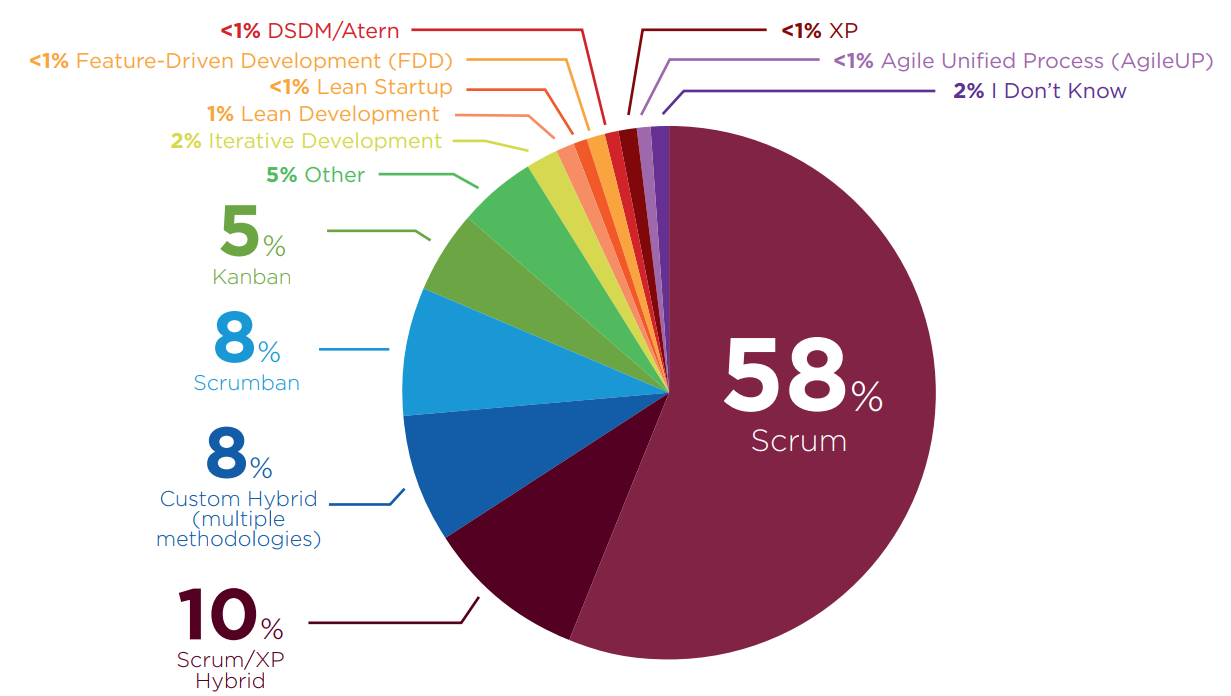
\includegraphics[width=1\textwidth]{5-AgileMethodologyUsed.png}
		\caption{Most used agile methodologies}{Source: The \emph{11th annual state of agile survey}}
		\label{fig:5-AgileMethodologyUsed}
	\end{center}
\end{figure}

Now, a general description of \emword{Scrum} is exposed.


\subsection{Scrum}
\emword{Scrum} \cite{ScrumGuide} is an agile project management methodology not necessarily related with software projects. \emword{Scrum} has two main characteristics: The first one is that the development of the software is carried out in incremental iterations, whilst the second one is that coordination meetings are held throughout the project.
In \emword{Scrum}, the product is developed in series with a duration from one to four weeks called \emword{Sprints}. The different requirements are captured as elements of a list called \emword{product backlog} which is created at the beginning of the project. Figure \ref{fig:5-ScrumSprints} represents the complete \emword{Scrum} life cycle.

\begin{figure}[!h]
	\begin{center}
		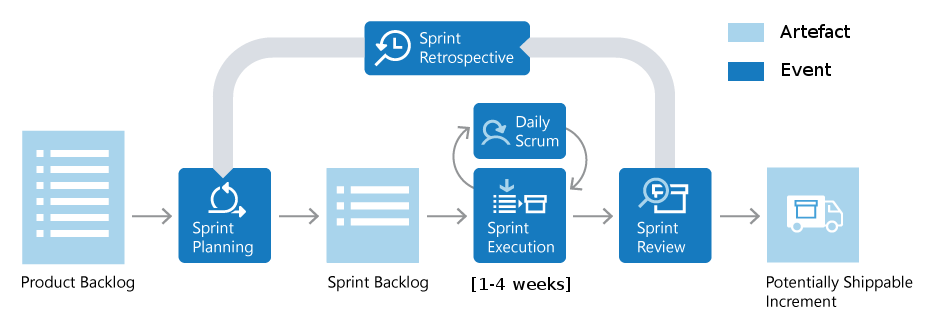
\includegraphics[width=1\textwidth]{5-ScrumSprints-v2.png}	
		\caption{Scrum life cycle}{Source: \url{https://www.visualstudio.com/es/learn/what-is-scrum}}
		\label{fig:5-ScrumSprints}
	\end{center}
\end{figure}


\subsubsection{Scrum Team} \label{5-ScrumTeam}
\emword{Scrum} Teams are self-organizing, cross-functional, non-distributed and must have an optimal size. The team model in \emword{Scrum} is designed to optimize flexibility, creativity, and productivity and its different roles are:

\begin{itemize}
	\item \emlst{Product owner.} The product owner is responsible for maximizing the value of the product and the work of the	development team. This person is also responsible of establishing the user stories, assigning them a priority and classifying them in the product backlog. The product owner must have a very clear perspective of the product which will be developed and must transmit it to the development team.
	
	\item \emlst{Scrum master.} The Scrum master is responsible for ensuring that the \emword{Scrum} is understood by all the members and that the \emword{Scrum} team adheres to \emword{Scrum} theory, practices, and rules. 
	
	\item \emlst{Development team.} The development team consists of professionals who do the work of delivering a potentially releasable increment of “Done” product at the end of each Sprint. It is recommended that they work full time, in the same place and they should not change during a Sprint.
\end{itemize}


\subsubsection{The Sprint}
In agile methodologies, the requirements that must fit the software which will be developed are collected into user stories. The user stories \cite{Coh04} are a brief description of the software functionality as the user perceives them. A Sprint is a time block with a duration from one to four weeks in which a product increment is obtained. Therefore, each Sprint can be considered as a project itself. A new Sprint starts immediately after the conclusion of the previous Sprint. The \emph{Sprint goal} is the objective set for the Sprint that can be met through the implementation of product backlog. No changes can be made in the Sprint goal during the Sprint execution. 


\subsubsection{Scrum events}
Some events are planned with a fixed duration and a concrete objective in order to minimize the need for meetings not defined previously. These events are the following ones:

\begin{itemize}
	\item \emlst{Sprint planning meeting.} It consists of a meeting carried out at the start of each Sprint where the elements from the product backlog to be developed are selected. Therefore, the Sprint backlog is created. This meeting should not last more than one day.
	
	\item \emlst{Daily Scrum.} It consists of daily meetings with a duration of less than fifteen minutes where the development team can synchronize their activities and create a plan for the next 24 hours. This is done by inspecting the work since the last daily Scrum and forecasting the work that could be done before the next one.
	
	\item \emlst{Sprint review.} It consists of a informal meeting held at the end of the Sprint to inspect the increment and adapt the product backlog if needed. During the Sprint review, the Scrum team and the stakeholders collaborate about what was done in the Sprint.
	
	\item \emlst{Sprint retrospective.} It is an opportunity for the Scrum team to inspect itself and create a plan for improvements to be enacted during the next Sprint. It has a maximum duration of three hours and takes place between the Sprint review meeting and the next Sprint planning meeting.
\end{itemize}


\subsubsection{Scrum artefacts}
When using \emword{Scrum}, some outputs are obtained known as \emword{Artefacts}. They represent work or value to provide transparency and opportunities for inspection and adaptation. Figure \ref{fig:5-ScrumSprints} shows the different artefacts and the moment in the Scrum life cycle when they are obtained.

\begin{itemize}
	\item \emlst{Product backlog.} It consists of an ordered list of requirements or user stories that will be included in the software product in the increments. This list, which is created by the Product owner, is never complete, therefore, it can change during the project to identify what the product needs. 
	
	\item \emlst{Sprint backlog.} It is a subset of the elements contained in the product backlog. It consists of an ordered list of user stories to be developed during this Sprint.
	
	\item \emlst{Product increment.} The increment is the sum of all the product backlog items that has been completed during a Sprint and add value to the increments of all the previous Sprints.
\end{itemize}

Heretofore, \emword{Scrum} project management methodology has been explained, besides the team needed for using it, the events organized and the artefacts produced. In the next section Kanban technique will be explained.


\section{Kanban}
Kanban \cite{Gar11,KS10} is a Japanese technique for managing the progress of the project. It was invented by Toyota and was used to control the progress of their work in the production line. Therefore, Kanban is not a specific software development technique, nevertheless, in the last few years it has been used in the management of software projects.

Kanban allows the development team to visualize the workflow of the different tasks. Normally, consists in using a slate board with three columns: \emph{To Do}, \emph{Doing} and \emph{Done}, that represents the different phases a task passes until it is completed. Each task in which a Sprint is divided is considered as a card which is put into the slate board. An example of this concept can be seen in Figure \ref{fig:5-KanbanBoard}.

To manage the Kanban Board, Trello is used, as it was previously indicated. This tool allows the creation of several boards. In each board many columns can be created with various tasks that can be moved from one column to another by means of a very friendly interface.

\begin{figure}[!h]
	\begin{center}
		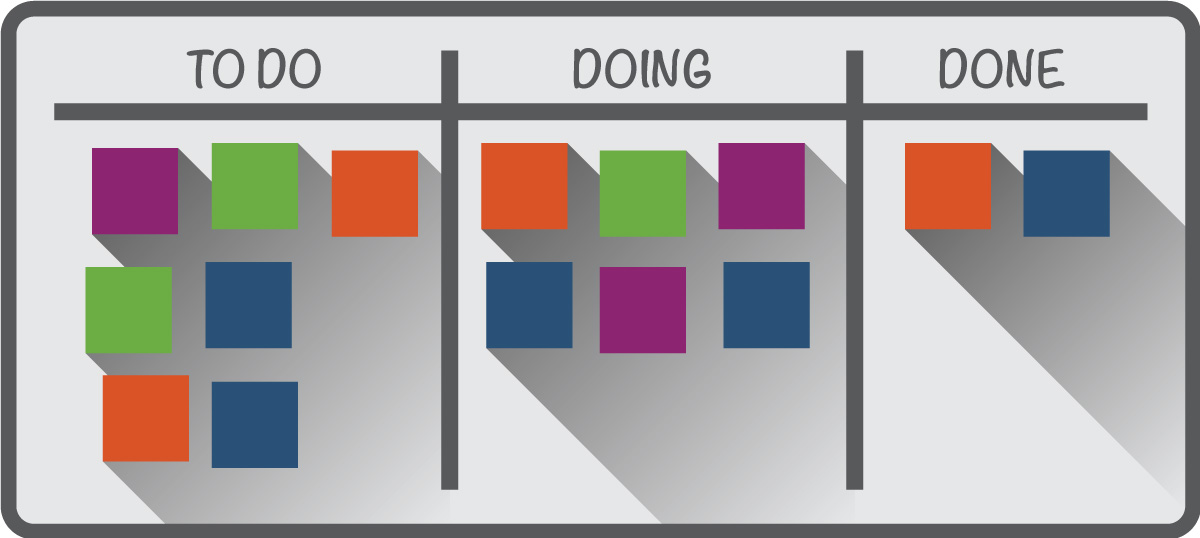
\includegraphics[width=0.8\textwidth]{5-KanbanBoard.jpg}
		\caption{Kanban Board}
		\label{fig:5-KanbanBoard}{Source: \url{www.qe2ingenieria.com}}
	\end{center}
\end{figure}

Up to this time, the project management methodology has been presented. Now, the development methodology will be introduced.


\section{Development methodology}
The development methodology is used by developers and engineers to write code, helping them in the process and giving some guidelines when developing computer systems in order to maintain a high code quality. In this \ac{BSc.} thesis the iterative and incremental software development methodology is used. In this method of software development the project is divided into several blocks, which match with the temporal blocks defined in \emword{Scrum} \cite{ItIncr}. 

Each iteration of the iterative and incremental methodology can be considered as a project itself where a value must be added to the final product. For each of those iterations all the tasks necessary to complete it must be executed, incorporating analysis, design, coding and testing phases (this is the reason of being called iterative). Moreover, in each iteration the team must take the work done in the previous iterations and include new objectives and requirements or improve the ones that are already accomplished (this is the reason of being called incremental). Figure \ref{fig:5-Iterative-and-incremental} represents the iterative and incremental methodology flow.

\begin{figure}[!h]
	\begin{center}
		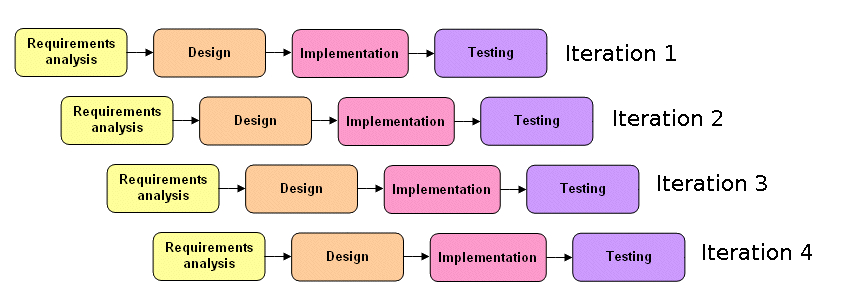
\includegraphics[width=0.9\textwidth]{5-Iterative-and-incremental.jpg}
		\caption{Iterative and incremental methodology flow}
		\label{fig:5-Iterative-and-incremental}{Adapted from  \url{http://www.technologyuk.net}}
	\end{center}
\end{figure}

Some of the advantages of using the iterative and incremental methodology are:
\begin{itemize}
	\item The final product is more adjusted to the client needs due to the fact that in each iteration part of the product is obtained and can be checked by the client. Therefore, some adjustments can be made in the following iterations.
	
	\item The changes that may appear during the project can be managed easier.
	
	\item Functional results are obtained from the firsts iterations.
	
	\item The client tends to involve itself more in the project. 
\end{itemize}

However, some disadvantages should be commented:
\begin{itemize}
	\item The result of each iteration must be a useful product, so that the result is really satisfactory for the client.
	
	\item Each of the steps in an iteration are fixed and iterations cannot be overlapped.
	
	\item Some techniques must be used in order to accomplish changes in the product easily, without incrementing the complexity of the project.
\end{itemize}


\section{Resources}
In this section we are going to describe the different technologies that are employed during the development of this \ac{BSc.} thesis.

\subsection{Hardware resources}
Now, the different hardware resources employed in the \ac{BSc.} thesis are detailed. These include the computer used to develop the \ac{BSc.} Thesis, the Raspberry Pi and the different peripherals attached to it. Figure \ref{fig:5-Foto_zulo} shows the different hardware resources before starting the project.


\begin{figure}[!h]
	\begin{center}
		\includegraphics[width=0.96\textwidth]{5-Foto_zulo.JPG}
		\caption{Hardware resources}
		\label{fig:5-Foto_zulo}
	\end{center}
\end{figure}


\begin{itemize}
	\item \emlst{Development computer.} The personal computer of the student has been employed for this purpose. The spec table is shown in Table \ref{tab:development-computer-spec-table}.
	
	\begin{table}[!h]
		\centering
		{\small
			\begin{tabular}{ |l|l|}
	\hline
	\rowcolor{tabheadbg}
	\multicolumn{2}{|c|}{\textscale{.8}{\textbf{Development computer (\emph{draco}) specs}}} \\
	\hline
	Model						& Asus Zeenbook UX430UA \\
	\hline
	Processor					& Intel® Core™ i7-7500U CPU at 2.70GHz $\times$ 4 \\
	\hline
	RAM memory 					& 8 GB \\
	\hline 
	Hard drive					& 512 GB HDD \\
	\hline
	First Operating System		& Ubuntu 16.04.3 LTS \\
	\hline
	Second Operating System		& Windows 10 \\
	\hline

\end{tabular}
		}
		\caption{Development computer spec table}
		\label{tab:development-computer-spec-table}
	\end{table}
	
	\item \emlst{Raspberry Pi 3.} The Raspberry Pi is a low cost, credit-card sized computer. The Raspberry Pi 3 is the third-generation Raspberry Pi. Table \ref{tab:raspberry-pi3-spec-table} shows its spec table. With this computer a memory card is also needed. The one used is the \emph{Samsung SDHC EVO 8gb Class 10+}.
	
	\begin{table}[!h]
		\centering
		{\small
			%\begin{tabular}{ |l|l|l|}
%	\hline
%	\rowcolor{tabheadbg}
%	\multicolumn{3}{|c|}{\textscale{.8}{\textbf{Raspberry Pi 3 Model B specs}}} \\
%	\hline
%	Price						& $\sim$35\euro{} \\
%	\hline
%	SoC							& Broadcom BCM2837 \\
%	\hline
%	Processor					& Quad Core ARM Cortex A53 (ARMv8) at 1.2GHz 64bit \\
%	\hline
%	RAM memory 					& 1 GB \\
%	\hline 
%	GPIO pins					& 40 \\
%	\hline
%	\multirow{7}{*}{External ports}
%		& HDMI \\ 
%		& CSI camera port \\ 
%		& DSI display port \\ 
%		& Micro SD port \\
%		& 4 $\times$ USB 2 ports \\
%		& Ethernet port \\
%		& Audio jack 3,5 mm \\
%	\hline
%	\multirow{2}{*}{Wireless connections}
%	& BCM43438 wireless LAN  \\ 
%	& Bluetooth Low Energy (BLE) \\
%	\hline
%
%\end{tabular}

\begin{tabular}{ |l|l|l|}
	\hline
	\rowcolor{tabheadbg}
	\multicolumn{3}{|c|}{\textscale{.8}{\textbf{Raspberry Pi 3 Model B specs}}} \\
			\hline
	Price                                 & $\sim$35\euro{}                                  & \multirow{14}{*}{
		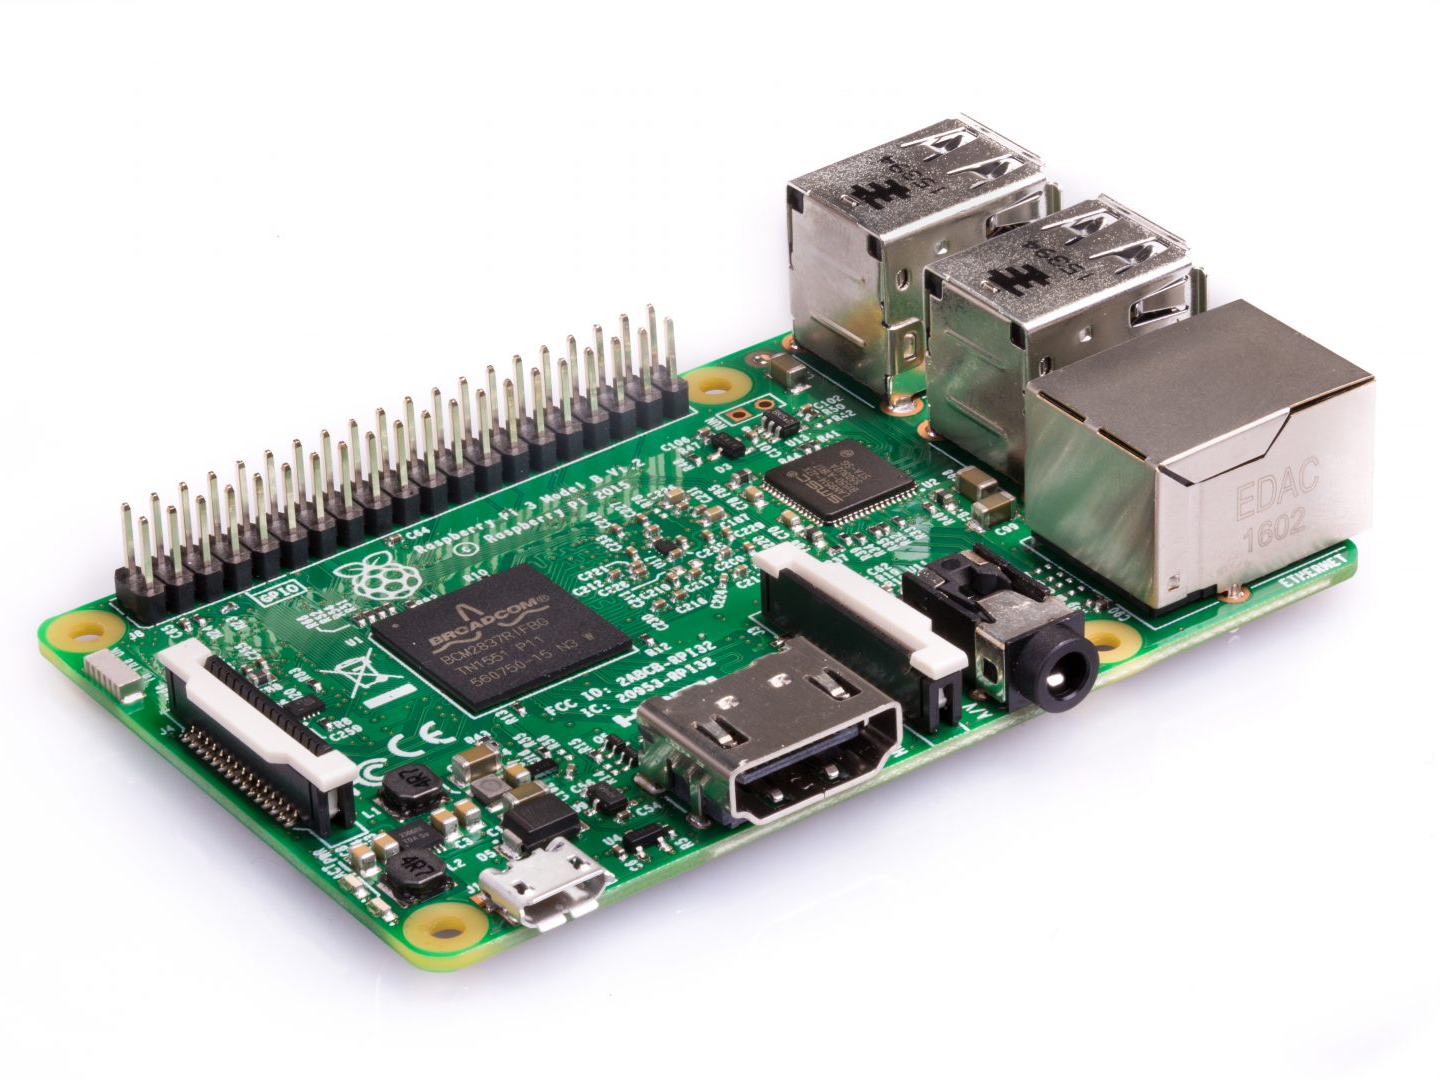
\includegraphics[width=0.36\textwidth]{5-RaspberryPi3.jpg}
	} \\ \cline{1-2}
	SoC                                   & Broadcom BCM2837                                 &                         \\ \cline{1-2}
	Processor                             & Quad Core ARM Cortex A53 				 &                         \\ 
			                              & (ARMv8) at 1.2GHz 64bit 								 &                         \\ \cline{1-2}
	RAM memory                            & 1 GB                                             &                         \\ \cline{1-2}
	GPIO pins                             & 40                                               &                         \\ \cline{1-2}
	\multirow{7}{*}{External ports}       & HDMI                                             &                         \\
	& CSI camera port                                  &                         \\
	& DSI display port                                 &                         \\
	& Micro SD port                                    &                         \\
	& 4 × USB 2 ports                                  &                         \\
	& Ethernet port                                    &                         \\
	& Audio jack 3,5 mm                                &                         \\ \cline{1-2}
	\multirow{2}{*}{Wireless connections} & BCM43438 wireless LAN                            &                         \\ \cline{2-2}
	& Bluetooth Low Energy (BLE)                       &                         \\ \hline
	
	
\end{tabular}

		}
		\caption{Raspberry Pi 3 spec table}
		\label{tab:raspberry-pi3-spec-table}
	\end{table}
	
	\item \emlst{Raspberry Pi Camera Module V2 \cite{PiCameraDoc}.} It is a hardware module that allows the Raspberry Pi to capture pictures and record videos using the CSI port. The camera used is the \emph{PI NOIR CAMERA V2}.\footnote{More information in https://www.raspberrypi.org/products/pi-noir-camera-v2/} The table \ref{tab:raspberry-pi3-camera-specs} shows its specs. \label{itm:Pi-camera-module-v2}
	
	\begin{table}[!h]
		\centering
		{\small
			%\begin{tabular}{ |l|l|}
%	\hline
%	\rowcolor{tabheadbg}
%	\multicolumn{2}{|c|}{\textscale{.8}{\textbf{Pi NoIR Camera V2 specs}}} \\
%	\hline
%	Price						& $\sim$25\euro{} \\
%	\hline
%	Weight						& 3g \\
%	\hline
%	Resolution					& 8 Megapixels \\
%	\hline 
%	Dimensions					& 25$\times$24$\times$9 mm \\
%	\hline	
%	Sensor						& Sony IMX219 \\
%	\hline
%	\multirow{3}{*}{Video modes}
%		& 1080$\times$120p at 30 fps \\ 
%		& 720$\times$480p at 60 fps\\ 
%		& 640$\times$480p at 60$/$90 fps \\ 
%	\hline
%	Additional information		& No Infrared filter (NoIR) \\
%	\hline
%\end{tabular}

% Please add the following required packages to your document preamble:
% \usepackage{multirow}


\begin{tabular}{|l|l|l|}
	\hline
	\rowcolor{tabheadbg}
	\multicolumn{3}{|l|}{\textscale{.8}{\textbf{Pi NoIR Camera V2 specs}}}                       \\ \hline
	Price                        & $\sim$25\euro{}                     & \multirow{9}{*}{
		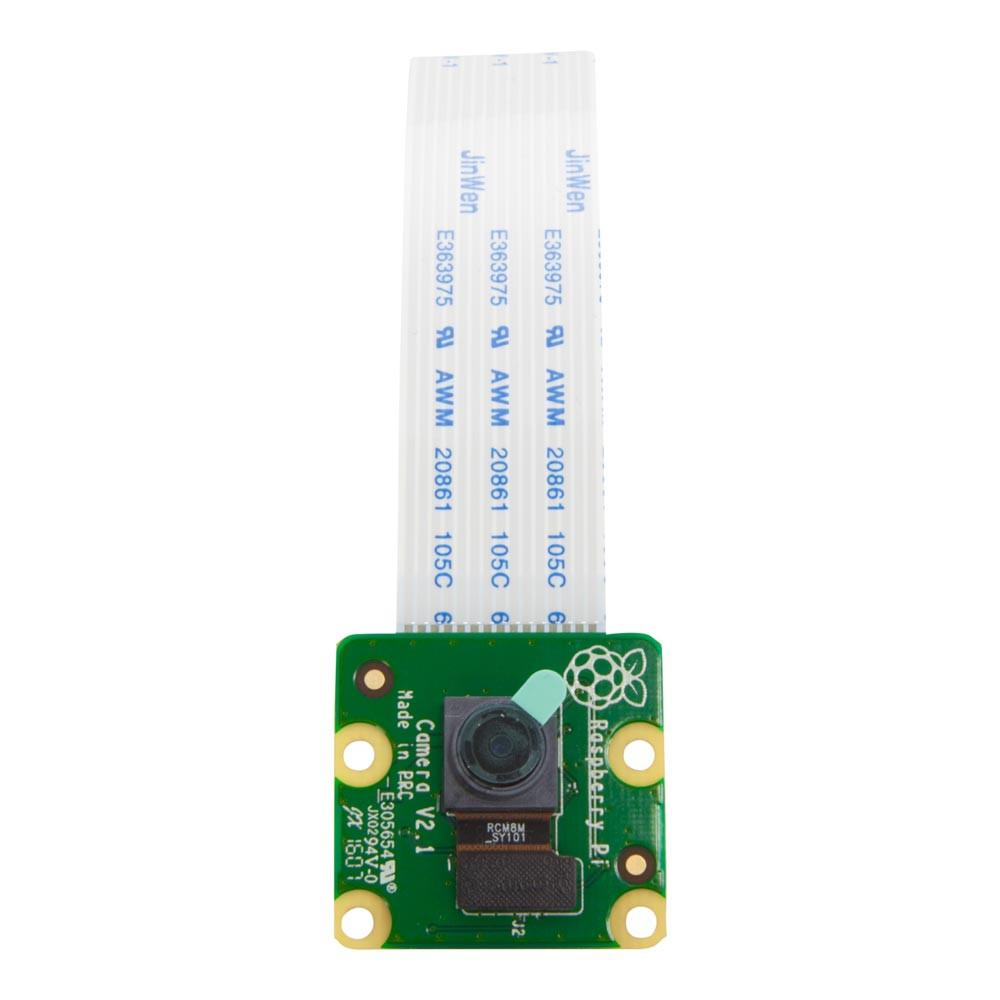
\includegraphics[width=0.28\textwidth]{5-PiCamera.jpg}
	} \\ \cline{1-2}
	Weight                       & 3g                        &                   \\ \cline{1-2}
	Resolution                   & 8 Megapixels              &                   \\ \cline{1-2}
	Dimensions                   & 25×24×9 mm                &                   \\ \cline{1-2}
	Sensor                       & Sony IMX219               &                   \\ \cline{1-2}
	\multirow{3}{*}{Video modes} & 1080p at 30 fps           &                   \\
	& 720p at 60 fps            &                   \\
	& 640x480p at 60/90 fps     &                   \\ \cline{1-2}
	Additional information       & No Infrared filter (NoIR) &                   \\ \hline
\end{tabular}
		}
		\caption{Pi NoIR Camera V2 spec table}
		\label{tab:raspberry-pi3-camera-specs}
	\end{table}

	\item \emlst{Sense HAT \cite{SenseHAT}.} It is an add-on board which is placed on top of the Raspberry Pi shield. It was made for the Astro Pi mission which took place in December 2015. This board is composed by several components: 8x8 RGB LED matrix, five-button joystick and some sensors (temperature, humidity, barometric pressure, magnetometer, accelerometer and gyroscope).
	
	\item \emlst{Power bank battery.} The Raspberry Pi board is going to be powered using a power bank battery. The one used has a capacity of 10000 mAh and provide a maximum amperage of 2.1 Ampers at 5 Volts.
	
	\item \emlst{MQ-7 Sensor. \cite{MQ7}} This sensor is able to measure Carbon Monoxide (CO) concentrations in the air. The MQ-7 can detect concentrations anywhere from 20 to 2000 ppm (parts per million) and has a fast response time. This sensor works with an input voltage of 5 volts and provide an analog output, therefore an anaglog to digital converter is needed.
	
	\item \emlst{MQ-2 Sensor \cite{MQ2}.} This sensor is able to measure methane, butane, petroleum gas, and smoke in concentrations between 300 and 10000 ppm. As the previous sensor, this one also works with a voltage of 5 volts and provides an analog output.
	
	\item \emlst{Analog-to-digital-converter \cite{ADC}.} \ac{ADC} is a system that converts an analog signal into a digital signal. Therefore, the input analog current is converted to a digital number proportional to the magnitude of the current which can be understood by a digital system.	
	
	\item \emlst{LM317 \cite{LM317}.} An electronic device which is capable of supplying more than 1.5 Ampers over an output voltage range form 1.25 to 37 Volts.
	
\end{itemize} 

\subsection{Software resources}
In this part the different software resources employed are described. These include the \ac{OS}, programming languages, libraries, the different development tools and the software used to generate the documentation as shown in Figure \ref{fig:5-SoftwareResources}.

\begin{figure}[!h]
	\begin{center}
		\includegraphics[width=0.92\textwidth]{5-SoftwareResources.pdf}
		\caption{Software resources}
		\label{fig:5-SoftwareResources}
	\end{center}
\end{figure}

\textbf{Operating Systems:}
\begin{itemize}
	\item \emlst{Ubuntu 16.04.3 LTS.} Ubuntu is a popular \ac{OS} based on \ac{GNU}$/$Linux. Ubuntu is one of the most used Linux distributions and it is normally used for personal computers, but also for servers and \ac{IoT}. This \ac{OS} is used for developing the software in the student's computer.
	
	\item \emlst{Debian 9 “Stretch”.} Debian is also an \ac{OS} based on \ac{GNU}$/$Linux. Debian has a big community form by developers and users, which maintain the software. It is also used for developing the software and for making the documentation.
	
	\item \emlst{Raspbian.} Raspbian is a Debian-based \ac{OS} designed for running on the Raspberry Pi.
	
	
\end{itemize}

\textbf{Programming Languages:}
\begin{itemize}
	\item \emlst{Python 3 \cite{Dow12}.} Python is a high-level programming language. Python focuses on offering a simple syntax, as well as being an interpreted language, allowing it to be ideal for scripting and for developing applications in various areas and for most platforms. In addition, it is an \ac{OO} language and has efficient and high-level data structures. Python has been used because it provides lot of support for Raspberry Pi devices. Moreover, the main libraries for the camera module of the Raspberry Pi are written in Python and can use the power of the NumPy scientific computation library.
	
	\item \emlst{HTML \cite{Duc11}.} Hypertext Markup Language or HTML is the most common markup language for the creation of webpages or web applications. Web browsers receive the HTML code from the web severs and render it into web pages that are displayed to the user.
	
	\item \emlst{CSS \cite{Duc11}.} Cascading Style Sheets or CSS is a style sheet language which is used to create rules that specify how the content of an element should appear in a web page.
	
	\item \emlst{JavaScript.} JavaScript or JS is a high-level interpreted programming language. It is commonly used in interactive webpages and it is a essential part of web applications. JS supports functional, imperative, object-oriented and event-driven programming styles. Initially, it was created to run on the client-side, but nowadays it is used also in the web servers.
	
\end{itemize}


\textbf{Database:}
\begin{itemize}
	\item \emlst{MySQL \cite{Bea05}.} MySQL is an open-source relational database management system. It uses \ac{SQL} language internally to access and manage the database.
	
	\item \emlst{MySQL Workbench.} It is an unified visual tool which provides data modelling, SQL development and comprehensive administrations tools for MySQL database servers configuration and maintenance.  
	
\end{itemize}

\newpage
\textbf{Libraries:}
\begin{itemize}
	\item \emlst{Python PiCamera \cite{PiCameraDoc}.} Python library for Python 2.7 or Python 3.2 (or above) which provides an interface for controlling the Raspberry Pi camera.
	
	\item \emlst{Python NumPy \cite{NumPy}.} NumPy is an open-source scientific computing package for Python. It provides an easy and efficient way of working with multidimensional structures, such as the matrices of motion vectors used by H.264/AVC video format which are employed by the PiCamera library.
	
	\item \emlst{Python Matplotlib \cite{Hun07}.} Matplotlib is a Python 2D plotting library which produces quality figures in a variety of formats. For simple plotting the \emph{pyplot} module provides a MATLAB-like interface.
	
\end{itemize}

\textbf{Development tools:}
\begin{itemize}
	\item \emlst{Atom.} Atom is a free open-source text and source coder editor for Linux, macOS, and Windows developed by GitHub. It allows to install a lot of plug-ins written in Node.js and has an embedded Git Control tool.\footnote{Available at \url{https://atom.io/}}
	
	\item \emlst{Vi.} Vi is a console text editor originally created for the Unix \ac{OS}. 
	
	\item \emlst{Git \cite{CS14}.} Git is a version control system for tracking changes in computer files and coordinating work on those files among multiple people. It is primarily used for source code management in software development, but it can be used to keep track of changes in any set of files.
	
	\item \emlst{GitHub.} GitHub is a web-based Git version control repository. It provides access control and several collaboration features such as bug tracking, feature requests, task management, and wikis for every project.\footnote{GitHub webpage: \url{https://github.com/}}	
	
\end{itemize}

\textbf{Software used for the documentation:}
\begin{itemize}
	\item \emlst{Trello.} Trello is a web tool which provides support for the Kanban technique allowing to manage the progress of the project. Trello provides the functionality to create boards composed by several lists with cards in them. For this project, a board has been created with three lists: \emph{To Do}, \emph{Doing} and \emph{Done}. Figure \ref{fig:5-Trello} shows a screen capture of Trello during the execution of User Story 3 in the Sprint 1.
	
	\begin{figure}[!h]
		\begin{center}
			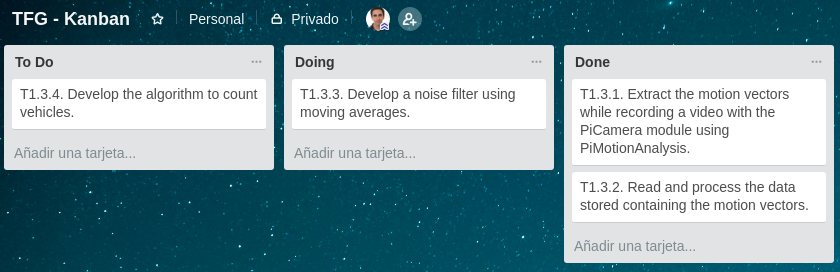
\includegraphics[width=0.96\textwidth]{5-Trello.png}
			\caption{Kanban board on Trello during the execution of User Story 3}
			\label{fig:5-Trello}
		\end{center}
	\end{figure}
	
	\item \emlst{\LaTeX{} \cite{Kot11}.} \LaTeX{} is a software for typesetting documents. It is not a word processor, but is used as a document markup language. \LaTeX{} is free, open source and provides great typographic quality on the documents, which makes it ideal for composing scientific documents. It is based on the \TeX{} typesetting engine created by Donald Knuth.
	
	\item \emlst{TeXstudio.} TeXstudio is a cross-platform and open source \LaTeX{} editor. TeXstudio has numerous features like syntax-highlighting, integrated viewer, reference checking, code folding and various assistants. Originally, TeXstudio was started as a fork of Texmaker that tried to extend it with additional features. 
	
	\item \emlst{esi-tfg \LaTeX{} class.} It is a \LaTeX{} class with allows to write the \ac{BSc.} thesis in a simple way, as its format conforms to the specification established for the \ac{BSc.} thesis by the \emph{Escuela Superior de Informática} from Ciudad Real. This class can be downloaded from the Arco Research Group Bitbucket page.\footnote{Available at \url{https://bitbucket.org/arco_group/esi-tfg}}
	
	\item \emlst{GIMP.} GIMP (\ac{GNU} Image Manipulation Program) is a free and open-source raster graphics editor used for image editing.
	
	\item \textbf{Inkscape.} It is an open-source editor which allows to create or edit vector graphics such as illustrations, charts, diagrams, etc. This tool is used for creating some of the figures of this document.
	
\end{itemize}

\textbf{Additional software:}
\begin{itemize}
	\item \emlst{MP4Box \cite{MP4Box}.} MP4Box is the multimedia package available in GPAC. It can be used for performing manipulations on multimedia files such as AVI, MPG, TS and ISO media files (for example MP4 or 3GP). In this work, it has been used to generate MP4 files from H.264 video format.
	
	\item \emlst{IBM Bluemix.} Bluemix is a cloud \ac{PaaS} developed by IBM. It integrates several services and programming languages, such as Java, Python, Node.js, GO, Ruby, etc. Bluemix is based on Cloud Foundry, which is an open-source multi cloud application originally developed by VMware.
	
\end{itemize}

% TFG - José Ángel Martín Baos. Escuela Superior de Informática. 2018
%%%% CHAPTER: Results %%%
\chapter{Results} % TODO
\label{chap:results}

\drop{I}{n} this chapter, the different results obtained during the execution of this \ac{BSc.} Thesis are presented. The working methodology presented in Chapter \ref{chap:methodology} is going to be used to carry out the work. In first place, the initial Sprint is presented, where the Scrum team will be set up, as well as the initial planning of the project. Subsequently, the different Sprints are presented, where the work planned in the initial Sprint will be carried out.




%%% Sprint 0
\section{Sprint 0: Initial planning}
In this first phase, Sprint 0, the main objective is to define the Scrum team, the user stories, the project plan, and the temporal and cost planning. Then, the draft (“Anteproyecto”) must be written. Once this Sprint has been completed, the project can start, as state in the temporal planning. The task associated to this initial Sprint can be shown in Table \ref{tab:Sprint0-Tasks}.

\begin{table}[hp]
	\centering
	{\small
		\begin{tabular}{|p{.7\textwidth}P{.1\textwidth}|}
	\hline
	\rowcolor{tabheadbg}
	\multicolumn{2}{|c|}{\textscale{.8}{\textbf{Sprint 0 tasks}}} \\
	\hline
	\hline
	\textscale{.8}{\textbf{Task}} 			& \textscale{.8}{\textbf{Estimate}} \\
	\hline
	Define the Scrum team					& 0,5h \\
	\hline
	Define the user stories					& 5h \\
	\hline
	Generate the project plan				& 2h \\
	\hline
	Generate the temporal planning			& 2h \\
	\hline
	Generate the cost planning				& 1h \\
	\hline
	Investigate about similar proposals								& 3h \\
	\hline
	Create a GitHub repository				& 0,5h \\
	\hline
	Write the draft (“Anteproyecto”)		& 21h \\
	\hline
	\textbf{Total} 							& 35h \\
	\hline

\end{tabular}
	}
	\caption{Sprint 0 tasks}
	\label{tab:Sprint0-Tasks}
\end{table}

\subsection{Scrum Team}
Following the scrum roles defined in Section \ref{5-ScrumTeam}, the Scrum team will have the following structure:
\begin{itemize}
	\item \textbf{Product Owner:} Ricardo García Ródenas
	\item \textbf{Scrum Master:} Luis Rodríguez Benítez
	\item \textbf{Development Team:} José Ángel Martín Baos
\end{itemize}

\subsection{Product Backlog}
\REDNOTE{... \& User Stories Table}
\begin{table}[hp]
	\centering
	{\small
		\begin{tabular}{ |P{.08\textwidth}p{.56\textwidth}P{.1\textwidth}P{.14\textwidth}|}
	\hline
	\rowcolor{tabheadbg}
	\multicolumn{4}{|c|}{\textscale{.8}{\textbf{User stories}}} \\
	\hline
	\textscale{.8}{\textbf{ID}}	& \textscale{.8}{\textbf{User history}}	& \textscale{.8}{\textbf{Priority}}	& \textscale{.8}{\textbf{Estimation (h)}} \\
	\hline
	1 	& Configure Raspberry Pi Architecture 										& High 		& 15 \\ 
	\hline
	2 	& Install PiCamera module in the Raspberry Pi								& High 		& 5 \\ 
	\hline	
	3 	& Develop an algorithm to calculate the vehicle flow		 				& High 		& 30 \\ 
	\hline
	4 	& Install environmental and gas sensors into Raspberry Pi					& High 		& 25 \\ 
	\hline
	5 	& Obtain and process data from the sensors									& High 		& 30 \\ 
	\hline
	6 	& Develop a comunication module using IBM IoT								& High 		& 15 \\ 
	\hline
	7 	& Receive sensor data from the Raspberry Pi and store it into a Database	& High 		& 12 \\ 
	\hline
	8 	& Integrate camera, sensors and comunication module into an unique program	& Medium	& 8 \\ 
	\hline
	9 	& Design a web page to monitor the data obtained by the Raspberry Pi devices	& High 		& 10 \\ 
	\hline
	10 	& Monitor in real time the data obtained by the devices and send an alert if the pollutant gases exceed a threshold																		& Medium 		& 20 \\ 
	\hline
	11 	& Display the historical data generated by the Raspberry Pi devices			& Low	& 20 \\ 
	\hline	

\end{tabular}
	}
	\caption{User stories}
	\label{tab:User-Stories}
\end{table}
	
The different user stories are presented its corresponding Sprints. Each user story is formed by the following fields:
\begin{itemize}
	\item \emlst{Sprint.} It indicates the Sprint number to which the user story belongs to.
	\item \emlst{Priority.} Priority given to the user story. It can take the values: low, medium and high.
	\item \emlst{Effort.} The estimated duration of the user story in hours. 
	\item \emlst{Name.} The label of the user story.
	\item \emlst{Description.} It is a brief definition of the user story.
	\item \emlst{Tasks.} It consists in a list of the different tasks that must be executed to complete the user story.
	\item \emlst{Tests.} It is a list of the different tests defined for the user story using \ac{TDD} as it is stated in Chapter \ref{chap:methodology}.
\end{itemize}

\subsection{Project plan}
\REDNOTE{Different sprints and its associated user stories and time estimation. \\
What is the total duration of the \ac{BSc.} Thesis?}
\begin{table}[hp]
	\centering
	{\small
		\begin{tabular}{|P{.08\textwidth}p{.56\textwidth}P{.15\textwidth}P{.08\textwidth}|}
	\hline
	\rowcolor{tabheadbg}
	\multicolumn{4}{|c|}{\textscale{.8}{\textbf{Sprints}}} \\
	\hline
	\hline
	\textscale{.8}{\textbf{Sprint}}			& \textscale{.8}{\textbf{Name}}	& \textscale{.8}{\textbf{User stories}}	& \textscale{.8}{\textbf{Estimate}} \\
	\hline
	0 	& Initial planning		 	& - 	& 35h \\ 
	\hline
	1 	& Development a basic algorithm to calculate the flow of vehicles		 		 	& 1, 2, 3 	& 50h \\ 
	\hline
	2 	& Design of an environmental parameters monitoring system		 	& \REDNOTE{...} 	& \REDNOTE{X}h \\ 
	\hline

\end{tabular}
	}
	\caption{Sprints}
	\label{tab:Sprints}
\end{table}

\subsection{Temporal planning}
\REDNOTE{Using the project plan, translate it to a graph (Remember the “Anteproyecto”)}

\REDNOTE{ Check the duration of all the task and sprints.} %TODO: Check the duration of all the task and sprints

\REDNOTE{The project start in September}

% Ganttproject


\subsection{Cost planning}
To manage the costs for the development of this project, two tables has been elaborated. Table \ref{tab:Hardware-Costs} indicates the costs related with the hardware resources that must be purchase in order to execute the project. Moreover, some development cost must be taken into account, which are indicated in Table \ref{tab:Development-Costs}. For the purpose of calculating the salary of the developer, the \ac{UCLM} retributions table of labor contracts for research projects on 2017 has been used. Therefore, it has been considered that the developer will have “Tercera-O-II” category, meaning that its annual cost will be of $23.598,83$\euro{}

\begin{table}[hp]
	\centering
	{\small
		\begin{tabular}{ |p{.5\textwidth}P{.1\textwidth}r|}
	\hline
	\rowcolor{tabheadbg}
	\multicolumn{3}{|c|}{\textscale{.8}{\textbf{Hardware costs}}} \\
	\hline
	\hline
	\textscale{.8}{\textbf{Item}}	& \textscale{.8}{\textbf{Quantity}}	& \textscale{.8}{\textbf{Cost}} \\
	\hline
	Raspberry Pi 3 					& 2 	& 49\euro{} \\ 
	\hline
	Pi NoIR Camera V2 				& 2 	& 28\euro{} \\ 
	\hline
	Memory card Samsung SDHC
	EVO 8gb Class 10+ 				& 2		& 8\euro{} \\ 
	\hline
	Power bank battery 				& 2 	& 29\euro{} \\ 
	\hline
	Camera Case		 				& 2 	& 14\euro{} \\ 
	\hline
	Raspberry Pi Sense HAT			& 2 	& 42\euro{} \\ 
	\hline
	Stacking Header 40 PIN 			& 2 	& 7\euro{} \\ 
	\hline
	MQ7 Gas Sensor		 			& 2 	& 2.5\euro{} \\ 
	\hline
	MQ2 Gas Sensor 					& 2 	& 3\euro{} \\ 
	\hline
	MCP3008 AD Conversor			& 2 	& 9\euro{} \\ 
	\hline
	Prototype shield  				& 1 	& 1.5\euro{} \\ 
	\hline
	Wires 							& 1 	& 7\euro{} \\ 
	\hline
	LM317 							& 2 	& 1.75\euro{} \\ 
	
	\Xhline{2\arrayrulewidth}
	\textbf{TOTAL:} &  		& \textbf{395\euro{}} \\ 
	\hline

\end{tabular}

	}
	\caption{Hardware costs}
	\label{tab:Hardware-Costs}
\end{table}

\begin{table}[hp]
	\centering
	{\small
		\begin{tabular}{ |p{.1\textwidth}P{.1\textwidth}r|}
	\hline
	\rowcolor{tabheadbg}
	\multicolumn{3}{|c|}{\textscale{.8}{\textbf{Development costs}}} \\
	\hline
	\hline
	\textscale{.8}{\textbf{Sprint}}	& \textscale{.8}{\textbf{Hours}}	& \textscale{.8}{\textbf{Cost}} \\
	\hline
	0			& 35h 			& \REDNOTE{X}\euro{} \\ 
	\hline
	\REDNOTE{XXX}	& \REDNOTE{X}h 		& \REDNOTE{X}\euro{} \\ 
	
	
	\Xhline{2\arrayrulewidth}
	\textbf{TOTAL:} & \textbf{\REDNOTE{X}h} 		& \textbf{\REDNOTE{X}\euro{}} \\ 
	\hline
	
	% Coste: Regla de 3:
	%    12 meses  ---- 23.598,83 euros
	%    X  meses  ---- Y euros
	% Jornada completa: 35 horas semanales

\end{tabular}
	}
	\caption{Development costs}
	\label{tab:Development-Costs}
\end{table}



%%% Sprint 1
\section{Sprint 1: Development a basic algorithm to calculate the flow of vehicles}
According to the project plan, in this sprint, a basic algorithm to calculate the vehicle flow must be developed. This involves executing the task associated to the user stories 1, 2 and 3. This iteration aims to obtain a basic algorithm to count the number of cars that cross a street in a certain amount of time so as to obtain the vehicle flow. \REDNOTE{Then in Sprint X, it will be improved.} To be able to count the number of cars using the PiCamera, \emword{motion vectors} are used. Therefore, a study about this concept has been done before implementing the algorithm. But first, it is necessary to configure the Raspberry Pi architecture and to install the PiCamera. 

\subsection{Sprint planning meeting}
During the planning meeting, the different user stories addressed in this sprint has been analysed. Consequently, they have been divided into several tasks and tests. The three user stories can be shown in Tables from \ref{tab:Sprint1-User-story-1} to \ref{tab:Sprint1-User-story-3}.

\UserStoryTable{1}{1}{High}{15}
{Configure Raspberry Pi Architecture}
{The \ac{OS} and all the components must be installed and configured.}
{	\item Install and configure Raspbian \ac{OS}
	\item Install the necessary libraries
}{	\item Check if the system works correctly using SSH connection
	\item Check if python works
}

\UserStoryTable{2}{1}{High}{5}
{Install PiCamera into Raspberry Pi}
{The PiCamera module must be working and some sample videos should be recorded in order to check the camera.}
{	\item Install the PiCamera module
	\item Develop a program to record videos
}{	\item Check if the camera is working correctly
}

\UserStoryTable{3}{1}{High}{30}
{Develop a basic algorithm to calculate the vehicle flow}
{Development of a basic algorithm that counts the number of cars that go across a street and determines their direction.}
{	\item Study the functionality of the motion vectors in H264/AVC
	\item Extract the motion vectors when recording a video with the PiCamera module using PiMotionAnalysis
	\item Read and process the data stored containing the motion vectors
	\item Develop a noise filter using moving averages
	\item Develop the basic algorithm to counts the cars
}{	\item Check the correctness of the motion vectors extracted
	\item Compare the data before and after applying the noise filter
	\item Assess the performance of the traffic-counting algorithm
}


\subsection{Results of the development of the tasks}
\textbf{Install and configure Raspbian \ac{OS} and the necessary libraries}

The first step consist of the Raspbian \ac{OS} installation, its configuration, and the installation of the necessary libraries. These steps are explained in the Appendix \ref{chap:installation_guide}. Once installed, the functionality of the system has been checked using a SSH connection from the development computer to the Raspberry, in order to ease the access to the System. 

\textbf{Install the PiCamera module and develop a program to record videos}

The next step is connecting the PiCamera module and configuring it as stated in Appendix \ref{chap:installation_guide}. Now, the device looks like in the Figure \ref{fig:6-Sistema_v1}. 

\begin{figure}[!h]
	\begin{center}
		\includegraphics[width=0.8\textwidth]{6-Sistema_v1.jpg}
		\caption{Device structure with PiCamera installed}
		\label{fig:6-Sistema_v1}
	\end{center}
\end{figure}

A configuration file has been implemented which contains some variables that are used by several modules of the device. Hence, these values are stored only once and can be changed easily. The whole file is shown and explained in Appendix \ref{chap:user_manual}. The parameters related with the camera are shown in Listing \ref{lst:6-camera-config}.

\lstinputlisting[language=Python, firstline=1, texcl, caption = {Part of \texttt{config.py} file containing the camera parameters}, label = lst:6-camera-config]{code/6-camera-config.py}

To assure the correct functionality of the camera, some videos are recorded. For that purpose and following the examples provided in PiCamera documentation \cite{PiCameraDoc}, a script has been developed. This script is shown in Listing \ref{lst:6-camera-video-recording}. This script must wait two seconds to ensure the camera is initialized correctly, then the camera starts recording during 60 seconds (as it is defined in \texttt{config.py}) and finally the video is saved in the file \texttt{my\_video.h264} in h264 video format.

\lstinputlisting[language=Python, firstline=1, texcl, caption = {Sample recording with PiCamera script}, label = lst:6-camera-video-recording]{code/6-camera-video-recording.py}


\textbf{Extract the motion vectors when recording a video with the PiCamera module using PiMotionAnalysis and PiMotionArray}

The result of the previous task allows recording videos using the PiCamera. This task deals with the need of extracting the motion data from the videos. To achieve this task, \texttt{PiMotionAnalysis} class from \texttt{picamera.array} is used. While recording is in progress, the incoming motion data is converted into a numpy array and an analysis method is called with the resulting array passed as argument. This class can be extended and the analysis method can be overridden. Therefore, in this method, the motion vectors can be used to detect movement in the video.

\BLUENOTE{Due to the fact that this class is used when the video is being recorded, it is used in the final implementation but first, in order to realize the different test, another class is used instead. The reason is that in this early steps of the work, it is more interesting to have the videos with the motion data stored into files and use them at any time. Hence, \texttt{PiMotionArray} class is used, which converts the incoming motion data into a numpy array also, but the conversion its made when the recording has finished. The class generates a 3-dimensional numpy array organized as (frames, rows, columns) where rows and columns are the number of the rows and columns of the macro-block \REDNOTE{(reference to the explanation of a macro-block)} in the frame. There is an extra column in the motion vector data that is not going to be used. Then, the data is stored into a file. 
}

\begin{figure}[!h]
	\begin{center}
		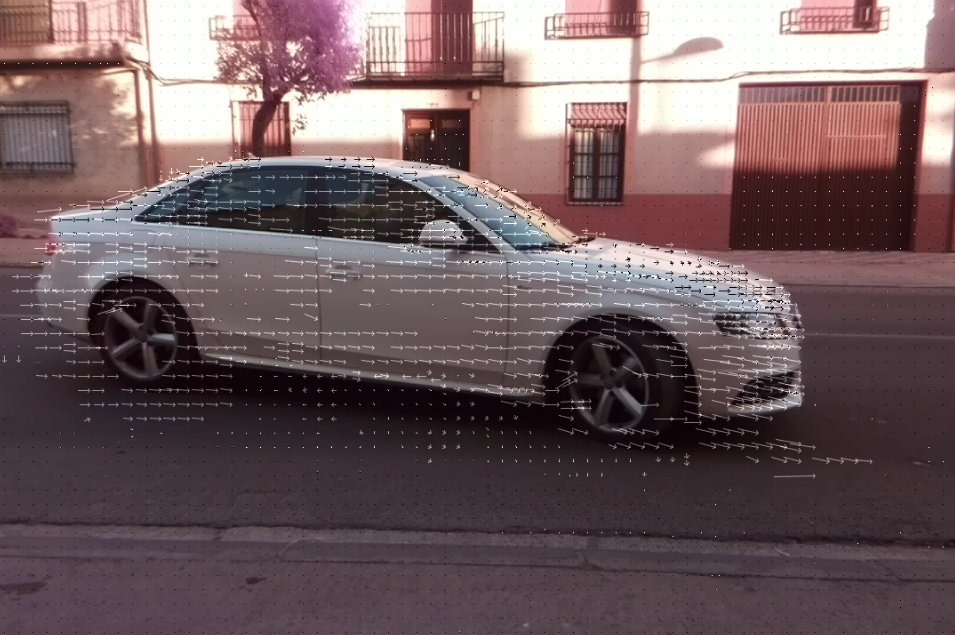
\includegraphics[width=0.8\textwidth]{6-Car_with_MV.png}
		\caption{Example of  the motion vectors taken by the Raspberry Pi}
		\label{fig:6-Car_with_MV}
	\end{center}
\end{figure}

The class used for recording the videos and the motion vectors used for developing the algorithm to count cars can be shown in Listing \ref{lst:6-Recorder-Sprint1}. Some parameters are given as arguments: \texttt{distance} and \texttt{angle}. They are used only for the filename so as to know afterwards the conditions of the camera when the video was recorded. In this class, the camera is configured according to the values stored in \texttt{config.py}. When the video has been recorded, it will be stored in a file with extension \texttt{.h264}, as well as the motion data, that will be stored in a file with the same name and extension \texttt{.data}. To finish with, the video will be also converted to \texttt{.mp4} to make easier its view in the development computer. 

\REDNOTE{IMPORTANT NOTE: Image resizer is not used. An other option is configure the camera resolution to 1920x1080 and use a resizer in the video to reduce the resolution given to the H.264 video coder.}

\lstinputlisting[language=Python, firstline=1, texcl, caption = {Class used to record a video and its corresponding motion data}, label = lst:6-Recorder-Sprint1]{code/6-Recorder-Sprint1.py}

\textbf{Develop a noise filter using moving averages}

There are some factors that can affect the number of motion vectors in a certain frame. Some of these factors can be the incorrect codification of that frame or a small object crossing the image (e.g., a person or a bug). Moreover, when H.264 video coding is used, there are several types of frame: I-frames, P-frames and B-frames \REDNOTE{(reference to their explanation)}. I-frames do not require other video frames to be decoded, therefore, they do not generate any motion vectors. Thus, the number of motion vectors in some frames is not going to be close to the reality, causing noise. To solve this problem, a smoothing technique is used. More concretely, simple moving averages calculation is applied.

A simple moving average \cite{Smi15} is a unweighted average of k prior values. Since a time series can be regarded as a sequence of values, $\{\overline {x_{t}}\}$, being $t=1,2,3,4,…n$, the moving average of these values can be computed. If we assume that $n$ is quite large, and we select an integer $k$ which is much smaller than $n$, we can compute the simple moving averages (of order k) as shown in Equation (\ref{eq:simple_moving_averages}).

\begin{equation} \label{eq:simple_moving_averages}
\overline { { x }_{ t } } =\frac { 1 }{ k } \sum _{ i=t-k+1 }^{ t }{ { x }_{ i } } ,\quad 2\le k\le n
\end{equation}

The result of applying the simple moving average over the data recorded previously can be shown in Figure \ref{fig:6-moving_averages}. Here, it can be appreciate how the graphic corresponding with the data before applying simple moving averages (black line) has some noise and sometimes it falls to 0. Additionally, it can be shown how the problem is decreased using this smoothing technique.

\begin{figure}[!h]
	\begin{center}
		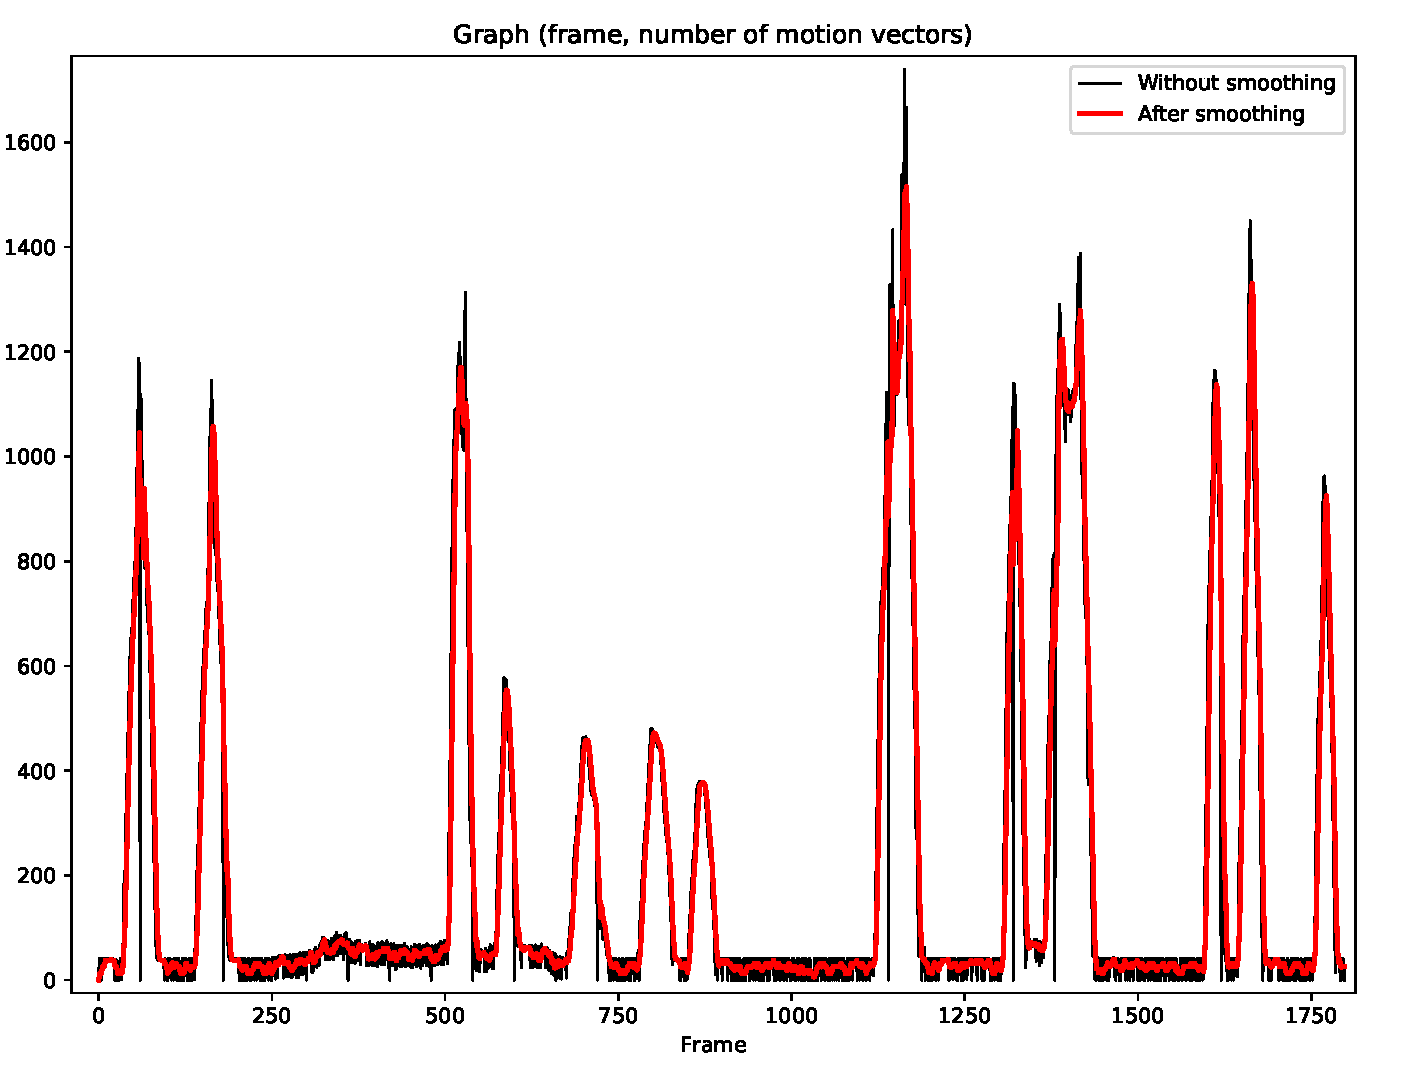
\includegraphics[width=1\textwidth]{6-moving_averages.pdf}
		\caption{Result of applying moving averages of order $n = 6$ to smooth the data}
		\label{fig:6-moving_averages}
	\end{center}
\end{figure}


\textbf{Develop the basic algorithm to counts the cars}

To count the cars that go across a street depending on its direction and using the motion data previously stored, an algorithm has been developed. Its pseudocode is shown in Algorithm \ref{alg:count_cars_V1}. This algorithm discriminates the cars direction (left or right). For each of the directions, the following algorithm is executed: 

For each frame, the number of motion vectors in that frame is compared with the number of vectors in the previous frame, increasing or decreasing a variable called \texttt{growth}. Once the number of frames exceed the \texttt{HEIGHT\_THRESHOLD} variable, if the \texttt{growth} variable is positive, the variable \texttt{n\_positive\_frames} is increased by one. If this last variable overtakes the \texttt{WIDTH\_THRESHOLD} variable, then we can consider that a new car has been detected. If the \texttt{growth} variable gets equal to \texttt{-GROWTH\_LIMIT}, then we consider that the car has already passed, and the variable \texttt{n\_positive\_frames} is restored to its initial value (zero).

An example of the execution fo the algorithm can be shown in Figure \ref{fig:6-Count_cars_graphic}, where the blue line represents the number of motion vectors with left direction for each frame, and the red line represents the same but for right direction. The black line, represent the \texttt{HEIGHT\_THRESHOLD} variable. Therefore, a car can be predicted if the number of frames in one direction overtakes the \texttt{HEIGHT\_THRESHOLD} variable during more than \texttt{WIDTH\_THRESHOLD} frames. And, it can be considered that the car has already cross if the number of frames has been decreasing $\texttt{GROWTH\_LIMIT} \times 2 $ frames, regardless if the number of motion vectors is under the \texttt{HEIGHT\_THRESHOLD} variable or not. Therefore, in Figure \ref{fig:6-Count_cars_graphic}, we can consider that two different cars have cross near the frame 1000, as the number of motion vectors has decreased during more than $\texttt{GROWTH\_LIMIT} \times 2 $ frames.

%\IncMargin{1em}
\begin{algorithm}
	\SetKwInOut{Input}{Input}\SetKwInOut{Output}{Output}
	\LinesNumbered
	\SetAlgoLined
	
	\Input{cols --> Number of colums with a macroblock in each frame\\
		rows --> Number of rows with a macroblock in each frame\\
		frames --> The number of frames in the video. \\
		motion\_data --> Array that contains a structure [x,y,SAD] for each frame} 
	\Output{n\_cars  --> Vector which contains the number of cars that has been counted crossing in left and right direction respectively.}
	
	n\_cars $\gets$ [0, 0]\;
	mv $\gets$ []\;
	smooth\_mv $\gets$ []\;
	car\_detected $\gets$ [False, False]\;
	growth $\gets$ [0, 0]\;
	n\_positive\_frames $\gets$ [0, 0]\;
	
	
	\For{frame $\gets$ 0 to frames}{
		%Add to the end of $mv$ vector a list with two elements. The first element consist in the number of motion vectors in that frame whose 'x' value is greather than the variable $GROUP\_SENSITIVITY$. The second element is the number of them whose 'x' value is lower than $-GROUP\_SENSITIVITY$.
		\tcc{Obtain number of motion vectors in each direction.}
		mv.append([ (motion\_data[frame]['x'] > GROUP\_SENSITIVITY).sum() ,
		(motion\_data[frame]['x'] < -GROUP\_SENSITIVITY).sum() ])\;
		
		\BlankLine
		\tcc{Apply moving averages to smooth the number of motion vectors}
		tmp\_left $\gets$ 0, tmp\_right $\gets$ 0\;
		\For{i $\gets$ 0 to SMOOT\_ORDER}{
			j $\gets$ frame - i\;
			\lIf{j < 0}{j $\gets$ 0}
			tmp\_left $\gets$ tmp\_left + mv[j][0] \;
			tmp\_right $\gets$ tmp\_right + mv[j][1]\;
		}
		smooth\_mv.append([tmp\_left / SMOOT\_ORDER, tmp\_right / SMOOT\_ORDER])\;
		
		\BlankLine
		\BlankLine
		\For{direction $\gets$ 0 to 2}{
			\uIf{smooth\_mv[frame-1][direction] < smooth\_mv[frame][direction]\\
				\hskip2em \textbf{and} growth[direction] < GROWTH\_LIMIT}{
				growth[direction] $\gets$ growth[direction] + 1\;
			}
			\ElseIf{smooth\_mv[frame-1][direction] < smooth\_mv[frame][direction]\\
				\hskip2em \textbf{and} growth[direction] > -GROWTH\_LIMIT}{
				growth[direction] $\gets$ growth[direction] - 1\;
			}
			
			\uIf{smooth\_mv[frame][direction] >= HEIGHT\_THRESHOLD \\
				\hskip2em \textbf{and} growth[direction] > 0}{
				n\_positive\_frames[direction] $\gets$ n\_positive\_frames[direction] + 1\;
				\If{n\_positive\_frames[direction] >= WIDTH\_THRESHOLD \\
					\hskip2em \textbf{and} car\_detected[direction] = False}{
					car\_detected[direction] $\gets$ True\;
					n\_cars[direction] $\gets$ n\_cars[direction] + 1\;
				}
				
			}
			\ElseIf{growth[direction] = -GROWTH\_LIMIT}{
				car\_detected[direction] $\gets$ False\;
				n\_positive\_frames[direction] $\gets$ 0\;
			}	
		}	
	}
	\caption{Count cars (First Version)}\label{alg:count_cars_V1}
\end{algorithm}\DecMargin{1em}

\begin{figure}[!h]
	\begin{center}
		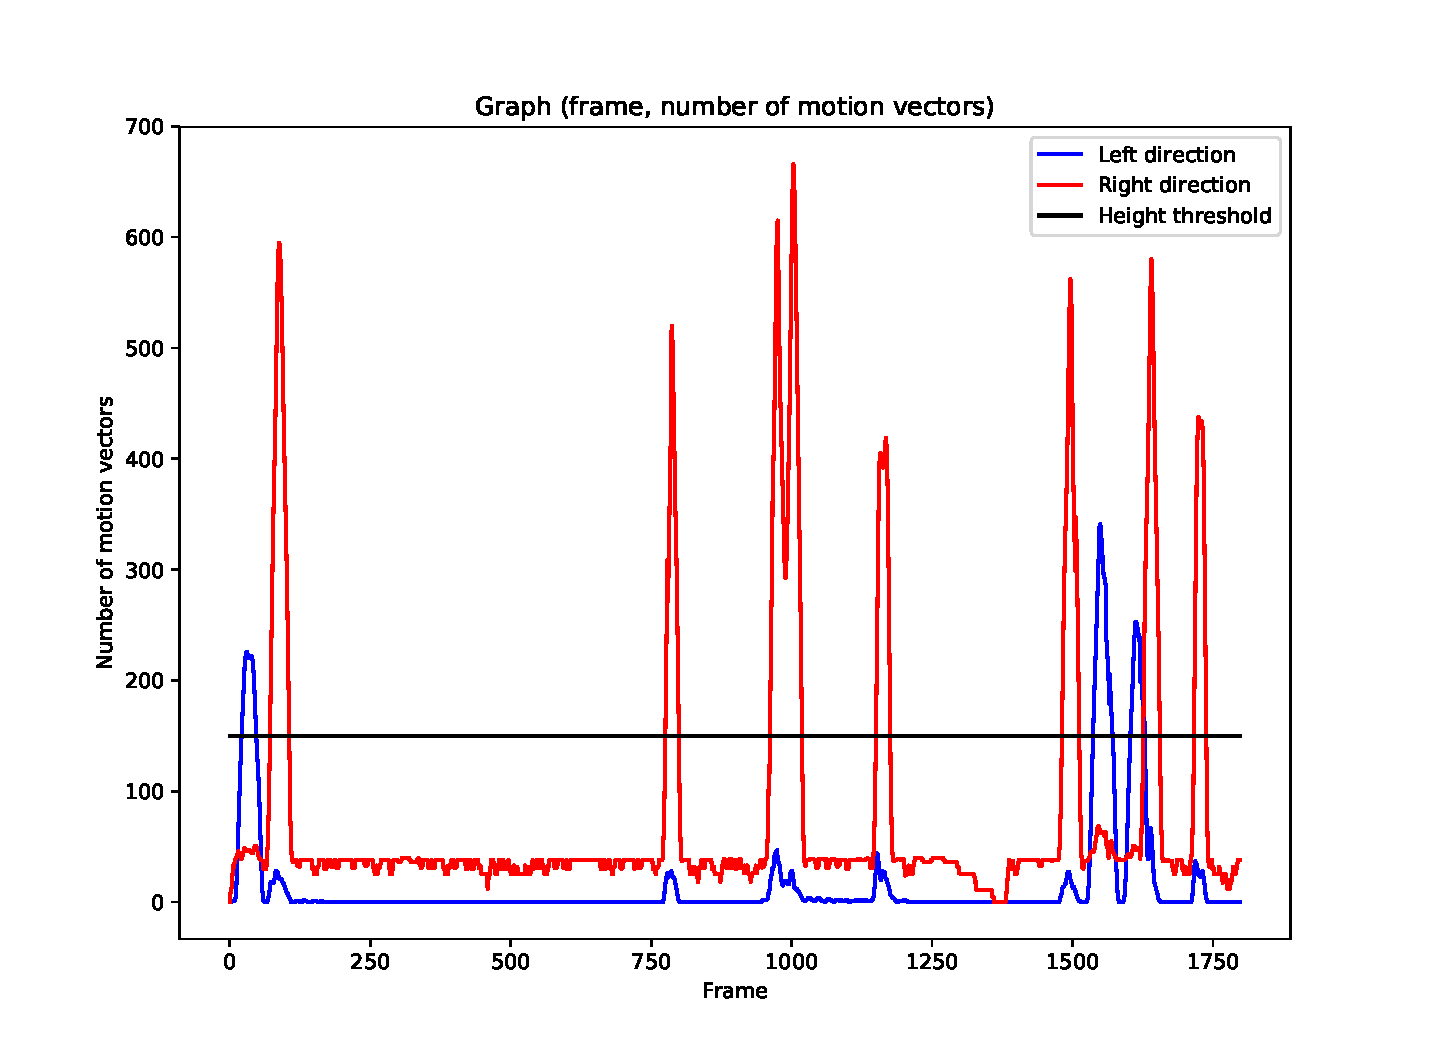
\includegraphics[width=1\textwidth]{6-Count_cars_graphic.pdf}
		\caption{Number of motion vectors in the test video 8}
		\label{fig:6-Count_cars_graphic}
	\end{center}
\end{figure}

Once the algorithm has been developed, it should be tested using the different videos recorded previously as it was stated in the list of test for the user story. The result of executing the algorithm over the different videos is shown in Table \ref{tab:Results_CountCars_V1}. After evaluating the results obtained, it is concluded that they are acceptable for the goal of this Sprint, therefore, a new Sprint can be started.

\begin{table}[hp]
	\centering
	{\small
		\begin{tabular}{ |P{.08\textwidth}P{.15\textwidth}P{.15\textwidth}P{.2\textwidth}P{.15\textwidth}|}
	\hline
	\rowcolor{tabheadbg}
	\multicolumn{5}{|c|}{\textscale{.8}{\textbf{Algorithm \ref{alg:count_cars_V1} results}}} \\
	\hline
	\hline
	\textscale{.8}{\textbf{Number}} & \textscale{.8}{\textbf{Quality}} & \textscale{.8}{\textbf{Camera angle}} & \textscale{.8}{\textbf{Distance to the road}} & \textscale{.8}{\textbf{Percentage of hits}} \\
	\hline
	1 	& 1080x720		 	&  center 		& 1m	& \textbf{100\%} \\ 
	\hline
	2 	& 1080x720		 	&  center 		& 1m	& \textbf{100\%} \\ 
	\hline
	3 	& 1080x720		 	&  center 		& 1m	& \textbf{90\%} \\ 
	\hline
	4 	& 1080x720		 	&  center 		& 2m	& \textbf{90.91\%} \\ 
	\hline
	5 	& 1080x720		 	&  center 		& 2m	& \textbf{100\%} \\ 
	\hline
	6 	& 1080x720		 	&  center 		& 2m	& \textbf{100\%} \\ 
	\hline
	7 	& 1080x720		 	&  center 		& 2m	& \textbf{94.74\%} \\ 
	\hline
	8 	& 1080x720		 	&  center 		& 3m	& \textbf{100\%} \\ 
	\hline
	9 	& 1080x720		 	&  center 		& 3m	& \textbf{90.91\%} \\ 
	\hline
	10 	& 1080x720		 	&  left 		& 1m	& \textbf{86.67\%} \\ 
	\hline
	11	& 1080x720		 	&  left 		& 1m	& \textbf{100\%} \\ 
	\hline
	12 	& 1080x720		 	&  left 		& 1m	& \textbf{100\%} \\ 
	\hline
	13 	& 1080x720		 	&  left 		& 2m	& \textbf{100\%} \\ 
	\hline
	14 	& 1080x720		 	&  left 		& 2m	& \textbf{55.56\%} \\ 
	\hline
	15 	& 1080x720		 	&  left 		& 2m	& \textbf{73.33\%} \\ 
	\hline
	16 	& 1080x720		 	&  left 		& 2m	& \textbf{88.89\%} \\ 
	\hline
	17 	& 1080x720		 	&  right 		& 1m	& \textbf{66.67\%} \\ 
	\hline
	18 	& 1080x720		 	&  right 		& 1m	& \textbf{78.57\%} \\ 
	\hline
	19 	& 1080x720		 	&  right 		& 1m	& \textbf{90\%} \\ 
	\hline
	20 	& 1080x720		 	&  right 		& 2m	& \textbf{83.33\%} \\ 
	\hline
	21 	& 1080x720		 	&  right 		& 2m	& \textbf{91.67\%} \\ 
	\hline
	22 	& 1080x720		 	&  right 		& 2m	& \textbf{88.89\%} \\ 
	\hline
	23 	& 1080x720		 	&  right 		& 2m	& \textbf{90\%} \\ 
	\hline
	\hline
	\multicolumn{3}{|c|}{\textscale{.8}{\textbf{Total number of tests: }} 23} & \multicolumn{2}{|c|}{\textscale{.8}{\textbf{Global percentage of hits: }} \textbf{89.57\%}} \\
	\hline
	
\end{tabular}
	}
	\caption{Results of the Algorithm \ref{alg:count_cars_V1} over the first test dataset}
	\label{tab:Results_CountCars_V1}
\end{table}


\REDNOTE{Task: Create a module that use the counting algorithm to obtain the vehicle flow in real time (using PiMotionAnalysis) in this Sprint or in another one.}

\REDNOTE{Do we need to comment the different Scrum events?}



%%% Sprint 2
\section{Sprint 2: Design of an environmental parameters monitoring system}
\REDNOTE{...}
% Product Backlog refinement

\subsection{Sprint planning meeting}
\REDNOTE{...}

\UserStoryTable{4}{2}{High}{x}
{Name of the user story}
{A description of the user story}
{	\item Task A
	\item Task B
	\item Task C
}{	\item Test A
	\item Test B
}

%Table \ref{tab:Sprint2-User-story-4}

\subsection{Results of the development of the tasks}
\textbf{task something ...}

\REDNOTE{...}





%%% Sprint 3
\section{Sprint 3: ....}
\REDNOTE{Task: Create a module that use the counting algorithm to obtain the vehicle flow in real time (using PiMotionAnalysis) in this Sprint or in another one.}
\REDNOTE{...}
% Product Backlog refinement

\subsection{Sprint planning meeting}
\REDNOTE{...}

%\UserStoryTable{4}{3}{High}{x}
%{Name of the user story}
%{A description of the user story}
%{	\item Task A
%	\item Task B
%	\item Task C
%}{	\item Test A
%	\item Test B
%}

%Table \ref{tab:Sprint2-User-story-4}

\subsection{Results of the development of the tasks}
\textbf{task something ...}

\REDNOTE{...}

\subsection{Daily Scrum}
\REDNOTE{...}

\subsection{Sprint review}
\REDNOTE{...}

\subsection{Sprint retrospective}
\REDNOTE{...}

% TFG - José Ángel Martín Baos. Escuela Superior de Informática. 2018
%%%% CHAPTER: Conclusions %%%
\chapter{Conclusions}
\label{chap:conclusions} 

\drop{T}{his} chapter presents a summary of the different goals achieved during the execution of this \ac{BSc.} thesis. Moreover, it proposes possible future works and ideas to extend the project done.


\section{Goal achievements}

The main objective of this \ac{BSc.} thesis (defined in Section \ref{chap:main-objective}) was the design and development of a pollution and traffic surveillance system prototype. With its construction it has been demonstrated the technical viability of the system.

The main goal has been achieved through the completion of the four specific objectives planned at the initial stage of the project. Now the satisfaction of the different specific objectives is analysed.
\begin{itemize}
	\item \textbf{O.1.} This objective has been fulfilled during the Sprint 1. For the completion of this objective, an efficient algorithm to determine the traffic flow in a street was developed. This algorithm detect correctly about the 90\% of the vehicles, which makes this solution compatible with the objective pursued in the \ac{BSc.} thesis. Thanks to the use of motion vectors, which are generated by the H.264/AVC video encoder on the \ac{GPU}, the number of vehicles that circulates on a street was counted in real time consuming low \ac{CPU} resources (about the 10\% of the \ac{CPU}). The algorithm is executed approximately 14 times faster than the time available between frames. Therefore, the use of this approach allows to use an inexpensive embedded system such as the Raspberry Pi.
	
	\item \textbf{O.2.} The fulfilment of this objective was achieved during the Sprint 2. An electronic circuit was developed to integrate different sensors. Firstly, the correct integration of several environmental sensors such as temperature, humidity and pressure sensors was achieved. These sensors are very important in order to calculate the pollutants dissipation in some emission models. Secondly, the integration of the LPG sensor was completed. Nonetheless, the integration of the CO gas sensor presents a minor problem: the current needed to heat the sensor and dissipate the CO between samples is not the recommended one (5 volts). The reason is that the voltage regulator chip (LM317) has an internal consumption and, therefore, the 5 volts obtained from the Raspberry Pi device were decreased by this chip. A feasible solution is to connect this chip to an external power supply with a higher voltage, for instance 9 volts.
	
	\item \textbf{O.3.} This objective was completely fulfilled during the execution of the Sprint 3. Through the use of the IBM Watson IoT Platform the scalability property is added to the solution developed in this thesis, which allows to use the developed device massively on urban areas. This is a key goal of this project and \ac{IoT} systems in general.
	
	\item \textbf{O.4.} This objective was completed during the Sprint 4. A web page was built in order to allow the visualization of the data generated by every connected device. Moreover, this web page has been developed taking into account the affordance, usability, and visibility of the design in order to ease its use.
\end{itemize}


\section{Future work}
In this section some ideas to improve the prototype and to expand it are proposed. In addition, other domains where the development project can be applied are described.

\subsection{Prototype improvements}
Some improvements can be done to add some additional value to the prototype developed in this \ac{BSc.} thesis. The improvements may be the following:
\begin{itemize}
	\item An automatic parameter tuning of the vehicle detection algorithm can be developed. Using different machine learning and video analysis techniques the different thresholds and variables of the vehicle counting algorithm developed in Sprint 1 can be estimated. Therefore, these values can be calculated automatically when the device is placed in a new location, saving the time needed for trial and error estimation. 
	
	\item The correct calibration of the different gas sensors. The best method consist in locating the sensors into a closed box with a known concentration of the target gas, therefore, the sensor can be calibrated with that concentration. The recommended concentration required for the correct calibration can be found in the sensors documentation. 
	
	\item In this project it has been demonstrated that we can integrate any gas sensor into the developed device. Therefore, more pollutant gases (such as NO\textsubscript{2}, PM\textsubscript{10}, PM\textsubscript{2.5} or  SO\textsubscript{2}) can be measured by installing other type of sensors.
	
\end{itemize}


\subsection{Prototype expansion}
The developed device can be used as a basis for the design of a \ac{ITS}, such as the one proposed in Figure \ref{fig:7-Prototype_expansion_diagram}. In order to design an intelligent system to predict the pollutants concentrations, an emission mathematical model, such as the COPERT \cite{NS16} model, could be integrated into the system. This model would estimate the emissions according to the type of vehicle, the speed, and the operating time. Six different types of vehicles are defined by the model and, therefore, the type of the different vehicles counted should be determined. Two strategies could be used to determine the vehicle type: The first one consists in capturing the license plates of the vehicles that are detected and use this information to obtain some relevant data such as the type of vehicle. The second strategy consists in using an image analysis technique, such as edge detection along with a deep learning algorithm to determine the type of vehicle.

This system can recommend traffic actions to reduce the contamination predicted by the COPERT model. Some actions that can be taken by the system could be: closing the traffic or lowering the speed limits in some streets, restricting the traffic in some areas to a certain number of vehicles or to certain license plates, etc. In addition, the system can measure the improvements generated by the actions taken, obtaining some feedback. This feedback can be used by a reinforcement learning algorithm to improve future traffic control decisions of the system.

\begin{figure}[!h]
	\begin{center}
		\includegraphics[width=0.94\textwidth]{7-Prototype_expansion_diagram.pdf}
		\caption{Prototype of the proposed Intelligent Transport System}
		\label{fig:7-Prototype_expansion_diagram}
	\end{center}
\end{figure}


\subsection{Other domains where the project can be used}
The device developed in this \ac{BSc.} thesis can also be applied to other domains. For example, the device can be adapted to be used as a control system in factories. Then, the gas sensors can be used to determine the concentration of some gases that could be dangerous to humans. These gases can be produced due to the normal operation of some machines or can be caused by a gas leak. Therefore, it is important to monitor the air of some factories to avoid an overexposure to toxic gases. Moreover, the camera can be used to count the number of units produced by the machines and to determine, for example, if any unit has a defect.

Another example is to adapt the developed camera system to count pedestrians in public areas or travellers in public transports such as trains. These can be used to monitor the number of people in public areas or determine the people flow inside rail stations.


\quoteauthor{Ciudad Real, 27th June 2018}
\quoteauthor{José Ángel Martín Baos}



%%%% CHAPTER: Conclusiones %%%
\chapter{Conclusiones}
\label{chap:conclusiones}

\drop{E}{n} este capítulo se presenta un resumen de los diferentes objetivos logrados durante la realización del \ac{TFG}. Además, se proponen posibles trabajos futuros e ideas para ampliar el proyecto.

\section{Análisis de la consecución de los objetivos}
El objetivo principal de este \ac{TFG} (definido en la Sección \ref{chap:main-objective}) es el diseño y desarrollo de un prototipo de sistema de vigilancia de contaminación y tráfico. Con este trabajo se ha demostrado que el sistema propuesto es técnicamente viable.

El objetivo principal se ha logrado mediante la realización de cuatro objetivos específicos planificados en la primera etapa del proyecto. A continuación, la consecución de los diferentes objetivos específicos será analizada.

\begin{itemize}
	\item \textbf{O.1.} Este objetivo ha sido cumplido durante la realización del Sprint 1. Para ello, se ha desarrollado un algoritmo eficiente capaz de determinar el flujo de tráfico. Este algoritmo detecta aproximadamente el 90\% de los vehículos correctamente, lo que lo convierte en una solución compatible con el objetivo perseguido en el \ac{TFG}. Mediante el uso de vectores de movimiento, generados en la \ac{GPU} usando el codificador de video H.264/AVC, el número de vehículos que circulan por una calle pueden ser contados en tiempo real y consumiendo bajos recursos de la \ac{CPU} (aproximadamente el 10\%). Este algoritmo se ejecuta aproximadamente 14 veces más rápido que el tiempo del que se dispone entre frames. Por lo tanto, el uso de este enfoque permite el uso de un sistema empotrado de bajo coste como la Raspberry Pi.
	
	\item \textbf{O.2.} Este objetivo fue logrado durante el Sprint 2. Un circuito electrónico ha sido desarrollado para integrar los diferentes sensores. En primer lugar, se ha logrado la correcta integración de diferentes sensores ambientales como de temperatura, humedad y presión. Estos sensores son muy importantes para poder calcular la disipación de los contaminantes mediante modelos de emisiones. En segundo lugar, la integración del sensores de LPG y CO se ha realizado correctamente. Sin embargo, la integración del sensor de CO presenta un problema: la corriente necesaria para calentar el sensor y disipar el CO entre mediciones no es la recomendada (5 voltios). Esto se debe a que el chip regulador de tensión (LM317) tiene una deriva interna y, por lo tanto, los 5 voltios obtenidos del dispositivo Raspberry Pi son disminuidos. Una posible solución es conectar este chip a una fuente de electricidad con un voltaje superior, por ejemplo 9 voltios. 
	
	\item \textbf{O.3.} Este objetivo ha sido completado durante la ejecución del Sprint 3. Mediante el uso de IBM Watson IoT Platform se ha añadido la propiedad de escalabilidad a la solución desarrollada en este trabajo, lo que permite el uso de dispositivo desarrollado de manera masiva en zonas urbanas. Esto es un objetivo clave de este proyecto y de los sistemas \ac{IoT} en general.
	
	\item \textbf{O.4.} Este objetivo fue completado durante el Sprint 4 mediante la realización de una página web que permite la visualización de los datos generados por cada dispositivo conectado. Además, esta página web ha sido desarrollada teniendo en cuenta el \textit{affordance}, la usabilidad y la visibilidad del diseño para facilitar su uso.
\end{itemize}


\section{Trabajo futuro}
En esta sección se proponen algunas ideas para mejorar y expandir el prototipo propuesto. Además, se describen otros dominios donde el proyecto desarrollado puede ser aplicado.

\subsection{Mejora del prototipo}
Algunas mejoras pueden ser realizas para aportar un valor adicional al prototipo desarrollado en este \ac{TFG}. Estas mejoras pueden ser las siguientes:

\begin{itemize}
	\item Desarrollo de un sistema de calibración automática de los parámetros del algoritmo de detección de vídeo. Usando diferentes técnicas de machine learning y análisis de vídeo se pueden calcular los diferentes umbrales y variables necesarias para el algoritmo de conteo de vehículos desarrollado en el Sprint 1. Por lo tanto, estos valores pueden ser calculados automáticamente cuando el dispositivo se coloca en una nueva localización, ahorrando el tiempo necesario para una calibración mediante prueba y error.
	
	\item Calibrar los sensores de gas de manera precisa. El mejor método para lograrlo consiste en colocar el sensor en un recipiente cerrado con una concentración de gas previamente conocida, de forma que el sensor se pueda calibrar usando esa concentración. En la documentación de los sensores se encuentra detallada la concentración recomendada para la correcta calibración de cada sensor.
	
	\item En este \ac{TFG} se ha demostrado que se puede integrar cualquier sensor de gas en el dispositivo desarrollado. Además, se pueden medir más tipos de gases contaminantes mediante la instalación del sensor correspondiente. Ejemplos de gases que podrían medirse son el NO\textsubscript{2}, PM\textsubscript{10}, PM\textsubscript{2.5} o  SO\textsubscript{2}.
	
\end{itemize}


\subsection{Expansión del prototipo}
El dispositivo desarrollado puede ser usado como base para el diseño de un Sistema Ingeligente de Transporte, como el propuesto en la Figura \ref{fig:8-Diagrama_expansión_prototipo}. Para poder desarrollar un sistema inteligente que sea capaz de predecir la concentración de los contaminantes se necesita integrar un modelo de emisiones matemático, como el modelo COPERT \cite{NS16}. Este modelo estima las emisiones dependiendo del tipo de vehículo, su velocidad y el tiempo de funcionamiento. En el modelo se definen seis tipos diferentes de vehículos, por lo tanto se debe determinar el tipo de cada vehículo contado. Para esto se pueden usar dos estrategias: La primera consiste en capturar las matrículas de los vehículos que son detectados y usar esta información para obtener información relevante, como por ejemplo el tipo de vehículo. La segunda estrategia consiste en usar técnicas de análisis de imagen, como por ejemplo detección de bordes, junto con un algoritmo de \textit{deep learning} para determinar el tipo de vehículo.

Este sistema puede recomendar acciones de tráfico para reducir la contaminación predicha por el modelo COPERT. Algunas de las acciones que podría  recomendar el sistema son: cerrar el tráfico o disminuir los límites de velocidad en algunas calles, restringir el tráfico en algunas áreas a un número determinado de vehículos o por un determinado subconjunto de matrículas, etc. Además, el sistema podría medir el efecto generado por cada una de las acciones tomadas, obteniendo de esta manera una retroalimentación. Esta información puede ser usada por un algoritmo de aprendizaje por refuerzo para mejorar la toma de futuras decisiones de control de tráfico.

\begin{figure}[!h]
	\begin{center}
		\includegraphics[width=0.94\textwidth]{8-Diagrama_expansion_prototipo.pdf}
		\caption{Prototipo del Sistema Inteligente de Transporte propuesto}
		\label{fig:8-Diagrama_expansión_prototipo}
	\end{center}
\end{figure}


\subsection{Otros dominios donde puede ser aplicado el proyecto}
El dispositivo desarrollado en este \ac{TFG} puede ser aplicado también a otros dominios. Por ejemplo, el dispositivo puede ser adaptado para ser usado como sistema de control en algunas fábricas. De esta manera, los sensores de gas se pueden usar para determinar la concentración de algunos gases que pueden ser peligrosos para los humanos. Estos gases pueden ser producidos mediante el funcionamiento normal de algunas máquinas o debidos a fugas de gas. Por lo tanto, es muy importante monitorizar el aire de algunas industrias de forma que se evite una sobreexposición de los trabajadores a gases tóxicos. Además, la cámara puede ser usada para contar el número de unidades producidas por las máquinas, o incluso para determinar si alguna unidad tiene un defecto.

Otro ejemplo es adaptar el módulo de la cámara desarrollado para contar peatones en zonas públicas o viajeros en medios de transporte como trenes. De esta manera se puede controlar el número de personas en determinadas zonas públicas o incluso determinar el flujo de viajeres dentro de estaciones de tren.

\quoteauthor{Ciudad Real, a 27 de Junio de 2018} 
\quoteauthor{José Ángel Martín Baos}



\appendix
\appendixtitle
% TFG - José Ángel Martín Baos. Escuela Superior de Informática. 2018
%%%% CHAPTER: Installation Guide %%%
% !TeX spellcheck = en_GB

\chapter{Installation guide} % TODO: Revise all
\label{chap:installation_guide}

\drop{I}{n} this appendix, the steps to install and configure the Raspberry Pi device in order to execute the software developed in this project are explained. Raspbian \ac{OS} \cite{Raspbian} is the Operative System that will be installed on the Raspberry Pi. Raspbian is an modification of Debian \ac{OS} for Raspberry Pi and ARM processors. In this installation guide, a GNU/Linux Operating System has been employed in the personal computer.


\section{Installation and configuration of Raspbian}
The first step to get the device working consists in the installation of the Raspbian Operating System and the configuration of the device to allow us access the Raspberry from another device using a wireless connection.

\subsection{Installation of Raspbian in a SD card}
There are two main alternatives to install Raspbian in the Raspberry Pi. The first one consists in downloading the \ac{OS} image and extracting it into the SD card, which is the method explained here. The second form, which is recommended for people with lower knowledge on Linux \ac{OS}, consists in downloading the NOOBS software. This software has to be copied into the SD card and when the Raspberry Pi is executed for the first time an installation process will be carried out and Raspbian will be installed. 

Raspbian \ac{OS} can be downloaded from the Raspberry Pi downloads page\footnote{Raspbian download page: \url{https://www.raspberrypi.org/downloads/raspbian/}}. Once downloaded, the following steps should be followed in order to have Raspbian properly working on the Raspberry Pi board:
\begin{enumerate}
	\item Download Raspbian and check the download. To check if the download has been correctly carried out, the following command has to be executed, where \emph{file.zip} is the downloaded file and \emph{hash\_value} is the SHA-1 value for the downloaded file which can be found on the download page.
\begin{console}
$ sha1sum file.zip | grep hash_value
\end{console} %$

	\item Now, the mirco-SD card can be inserted and mounted on the computer. Usually the card gets mounted automatically. The list of devices mounted on the computer is shown in the Figure \ref{fig:Appendix_df-h_command}. Here, it can be observed that the mirco-SD card correspond to the route \texttt{/dev/sdb1}. The command used is: 
\begin{console}
$ df -h
\end{console} %$
	\begin{figure}[!h]
		\begin{center}
			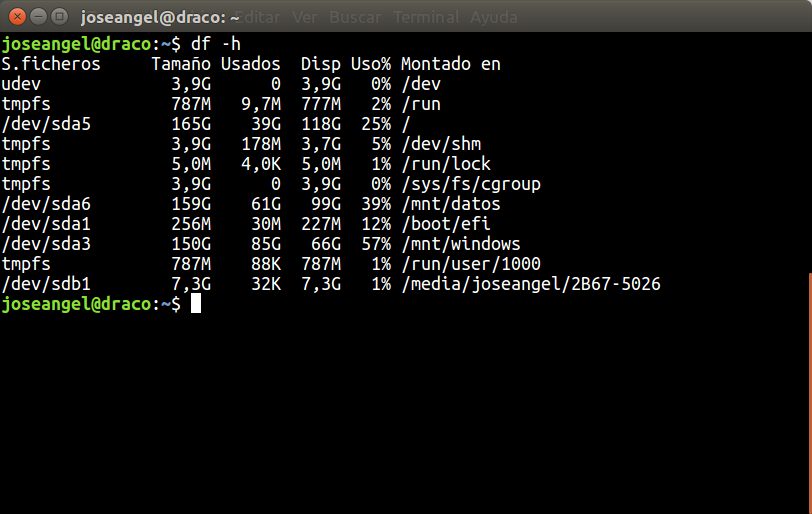
\includegraphics[width=0.9\textwidth]{Appendix_df-h_command.png}
			\caption{\texttt{df -h} command execution}
			\label{fig:Appendix_df-h_command}
		\end{center}
	\end{figure}

	\item Once the path where mirco-SD has been mounted is known, the next step is to execute the following command to unmount the card, where \texttt{/dev/sdb1} is de route corresponding to your card. This avoids that the \ac{OS} writes the card while the files are being copied.
\begin{console}
$ umount /dev/sdb1
\end{console} %$

	\item Now, the \ac{OS} image can be extracted and copied to the micro-SD card as shown in Figure \ref{fig:Appendix_SO_copy}. The following commands have to be executed from the directory where the file has been downloaded:
\begin{console}
$ unzip 2017-07-05-raspbian-jessie.zip 
$ sudo dd bs=4M if=2017-07-05-raspbian-jessie.img of=/dev/sdb1
\end{console} %$

	\begin{figure}[!h]
		\begin{center}
			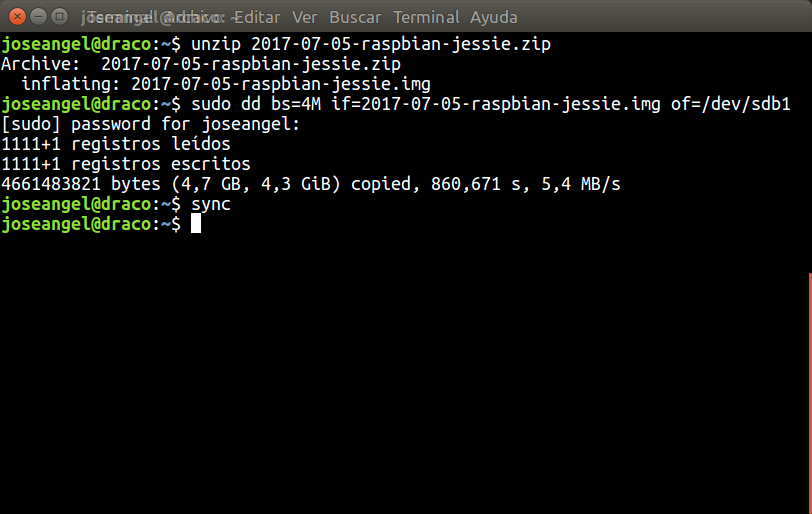
\includegraphics[width=0.9\textwidth]{Appendix_SO_copy.png}
			\caption{Console screenshot that shows the \ac{OS} copy process}
			\label{fig:Appendix_SO_copy}
		\end{center}
	\end{figure}

	\item Once the process has finished and before extracting the micro-SD card from the computer it should be ensured that the cache is clean. The next command must be executed:
\begin{console}
$ sync
\end{console} %$
	
\end{enumerate}


\subsection{Configuring Raspbian}
At this moment, the Raspbery Pi can be turned on. But firstly, it has to be connected to a external monitor or a TV using a HDMI cable. Nonetheless, this way is not very practical, therefore, some methods for allowing remote connection are explained. 

The first method consists in using \emph{ssh} protocol to access the Raspbery device. This protocol allows operating network services securely over an unsecured network. In others words, this method allows executing commands on the Raspberry Pi using a console, provided that the Raspberry Pi and the computer from where it is accessed are connected to the same network. OpenSSH tool \cite{OpenSsh} is installed with Raspbian \ac{OS} to provide the \emph{ssh} service. To activate it the following command should be executed:
\begin{console}
$ sudo raspi-config
\end{console} %$
This command executes the Raspbian configuration tool (Figure \ref{fig:Appendix_raspi-config_main}). \emph{Interfacing options} has to be selected. Using the new menu (Figure \ref{fig:Appendix_raspi-config_ssh}) SSH service should be selected and activated. Finally, the Raspberry Pi must be rebooted.

At this moment, the Raspberry Pi can be accessed from any computer connected to the same network using the next command, where \texttt{ipaddress} is the IP address of the network interface of the Raspberry Pi.
\begin{console}
$ ssh pi@ipaddress
\end{console} %$


The second method, consists in using a graphic remote session. VNC\footnote{VNC proyect main page: \url{http://www.hep.phy.cam.ac.uk/vnc_docs/index.html}} can be installed. VNC stands for Virtual Network Computing. It is, in essence, a remote display system which allows the user to view a computing 'desktop' environment, not only on the machine where it is running, but from anywhere on the Internet and from a wide variety of machine architectures. 

To activate VNC, the Interfacing options of the \texttt{raspi-config} tool has to be opened again as show in Figure \ref{fig:Appendix_raspi-config_ssh}. Then, VNC has to be selected and activated. Finally, the Raspberry Pi must be rebooted.

\begin{figure}[!h]
	\centering
	\subfigure[Main menu]{
		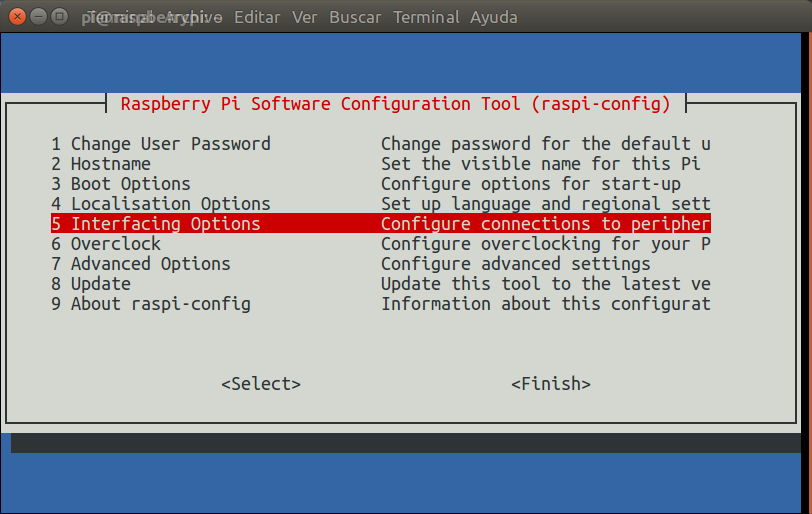
\includegraphics[width=0.48\textwidth]{Appendix_raspi-config.png}
		\label{fig:Appendix_raspi-config_main}
	}
	\subfigure[Interfacing Options]{
		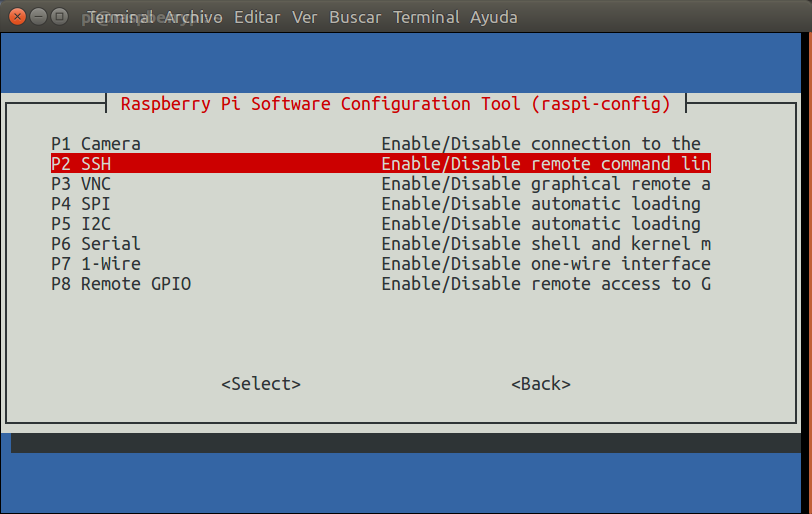
\includegraphics[width=0.48\textwidth]{Appendix_raspi-config_ssh.png}
		\label{fig:Appendix_raspi-config_ssh}
	}
	\caption{Screenshot of raspi-config tool}
	\label{fig:Appendix_raspi-config}
\end{figure}

To access the \textsc{vnc} server executing in the Raspberry Pi, we have opted for using \textsc{vnc} viewer for Google Chrome, which is a version of \textsc{vnc} Connect\footnote{RealVNC main page: \url{https://www.realvnc.com/en/}} application adapted to execute in Google Chrome web browser. A screenshot of the program can be shown in Figure \ref{fig:Appendix_VNC-Viewer-Chrome}.

\begin{figure}[!h]
	\begin{center}
		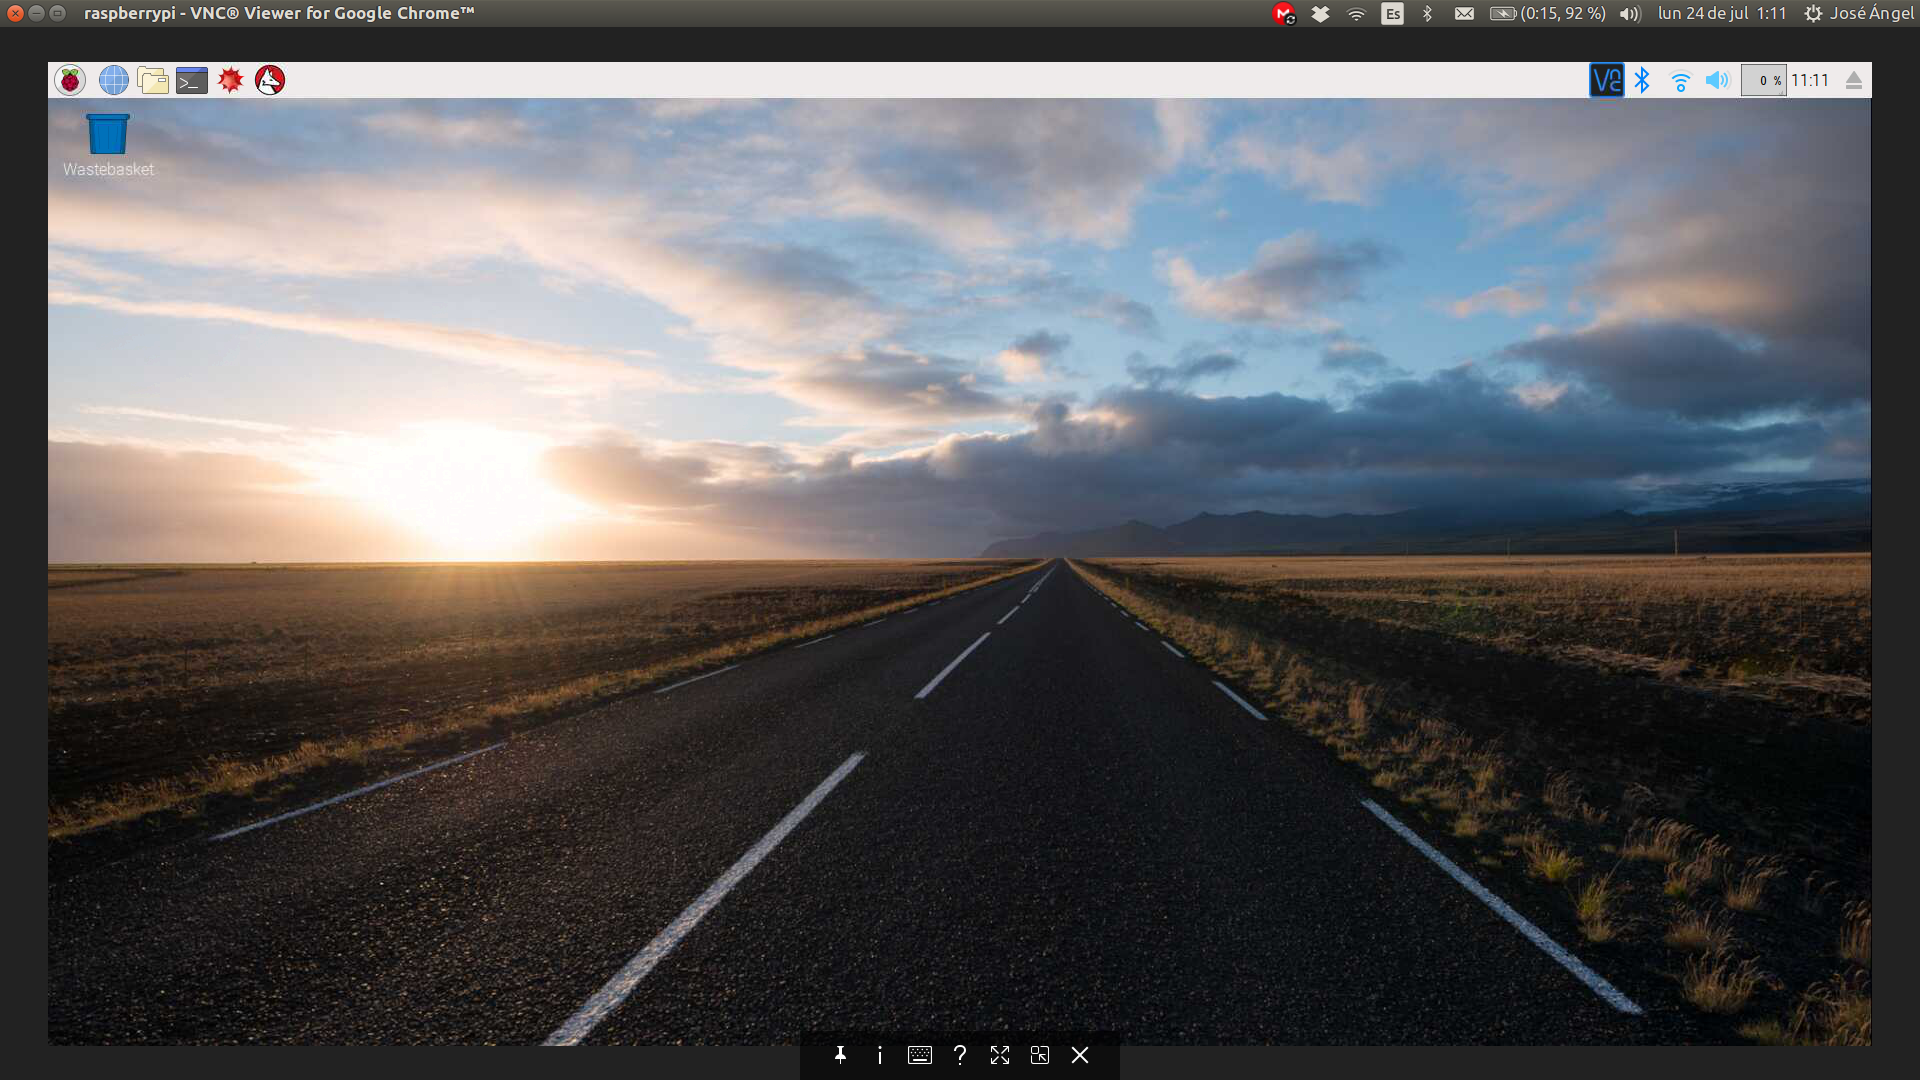
\includegraphics[width=1\textwidth]{Appendix_VNC-Viewer-Chrome.png}
		\caption{Screenshot of \textsc{vnc} Viewer for Google Chrome.}
		\label{fig:Appendix_VNC-Viewer-Chrome}
	\end{center}
\end{figure}

The last step in this configuration process is to update the Raspbian \ac{OS} and applications. To accomplish this task, first, the filesystem should be expanded. This means that all the free space in the SD card will be available to the \ac{OS}. Again, the raspberry configuration tool has to be executed (Figure \ref{fig:Appendix_raspi-config_main}), and the \emph{Advance Options} menu has to be opened. Then, the \emph{Expand Filesystem} option must be selected. To finish with, the following commands have to be executed to update Rasbian:
\begin{console}
$ sudo apt-get update
$ sudo apt-get upgrade
\end{console} %$


\section{Installation of the necessary hardware and software}
Once we have the Raspberry Pi configured, it is needed to install some basic software and configure the hardware. In this case, as Python 3 had been used to develop the program that runs into the Raspberry Pi, Python 3 package installer (known as PIP) is needed. This software allows to install Python 3 packages easily. The next command has to be executed:
\begin{console}
$ sudo apt-get install python3-pip
\end{console} %$

\subsection{Installation of the PiCamera module}
In this project, the \emph{Raspberry Pi camera module V2} \footnote{More information about the Raspberry Pi camera module can be found in: \url{https://www.raspberrypi.org/products/camera-module-v2/}} is used. PiCamera \cite{PiCameraDoc} library is used to manage the Raspberry Pi camera installed. This library can be found on the Raspbian repositories, so it can be installed easily using the \emph{apt-get} command:
\begin{console}
$ sudo apt-get install python3-picamera
\end{console} %$

The next step is to enable the camera connection. The raspberry configuration tool will be executed (Figure \ref{fig:Appendix_raspi-config_main}), and the \emph{Interfacing options} menu should be opened. There, \emph{Camera} must be selected and activated. Then, the system should be restarted. Is important to know that the camera may not work well if there is not at least 128 MB of memory asignated to the \textsc{gpu}.

The last step is to connect the camera to the Raspbery Pi. The \textsc{csi} port must be used for this purpose. This port is located between the \textsc{hdmi} port and the stereo plug. It is advisable that when the camera is being installed the Raspberry must be turned off to avoid any damage to the camera. When connecting it, the blue part of the bus must be facing the stereo plug and the Ethernet connection as it is shown in Figure \ref{fig:Appendix_camera_conection}. 

\begin{figure}[!h]
	\begin{center}
		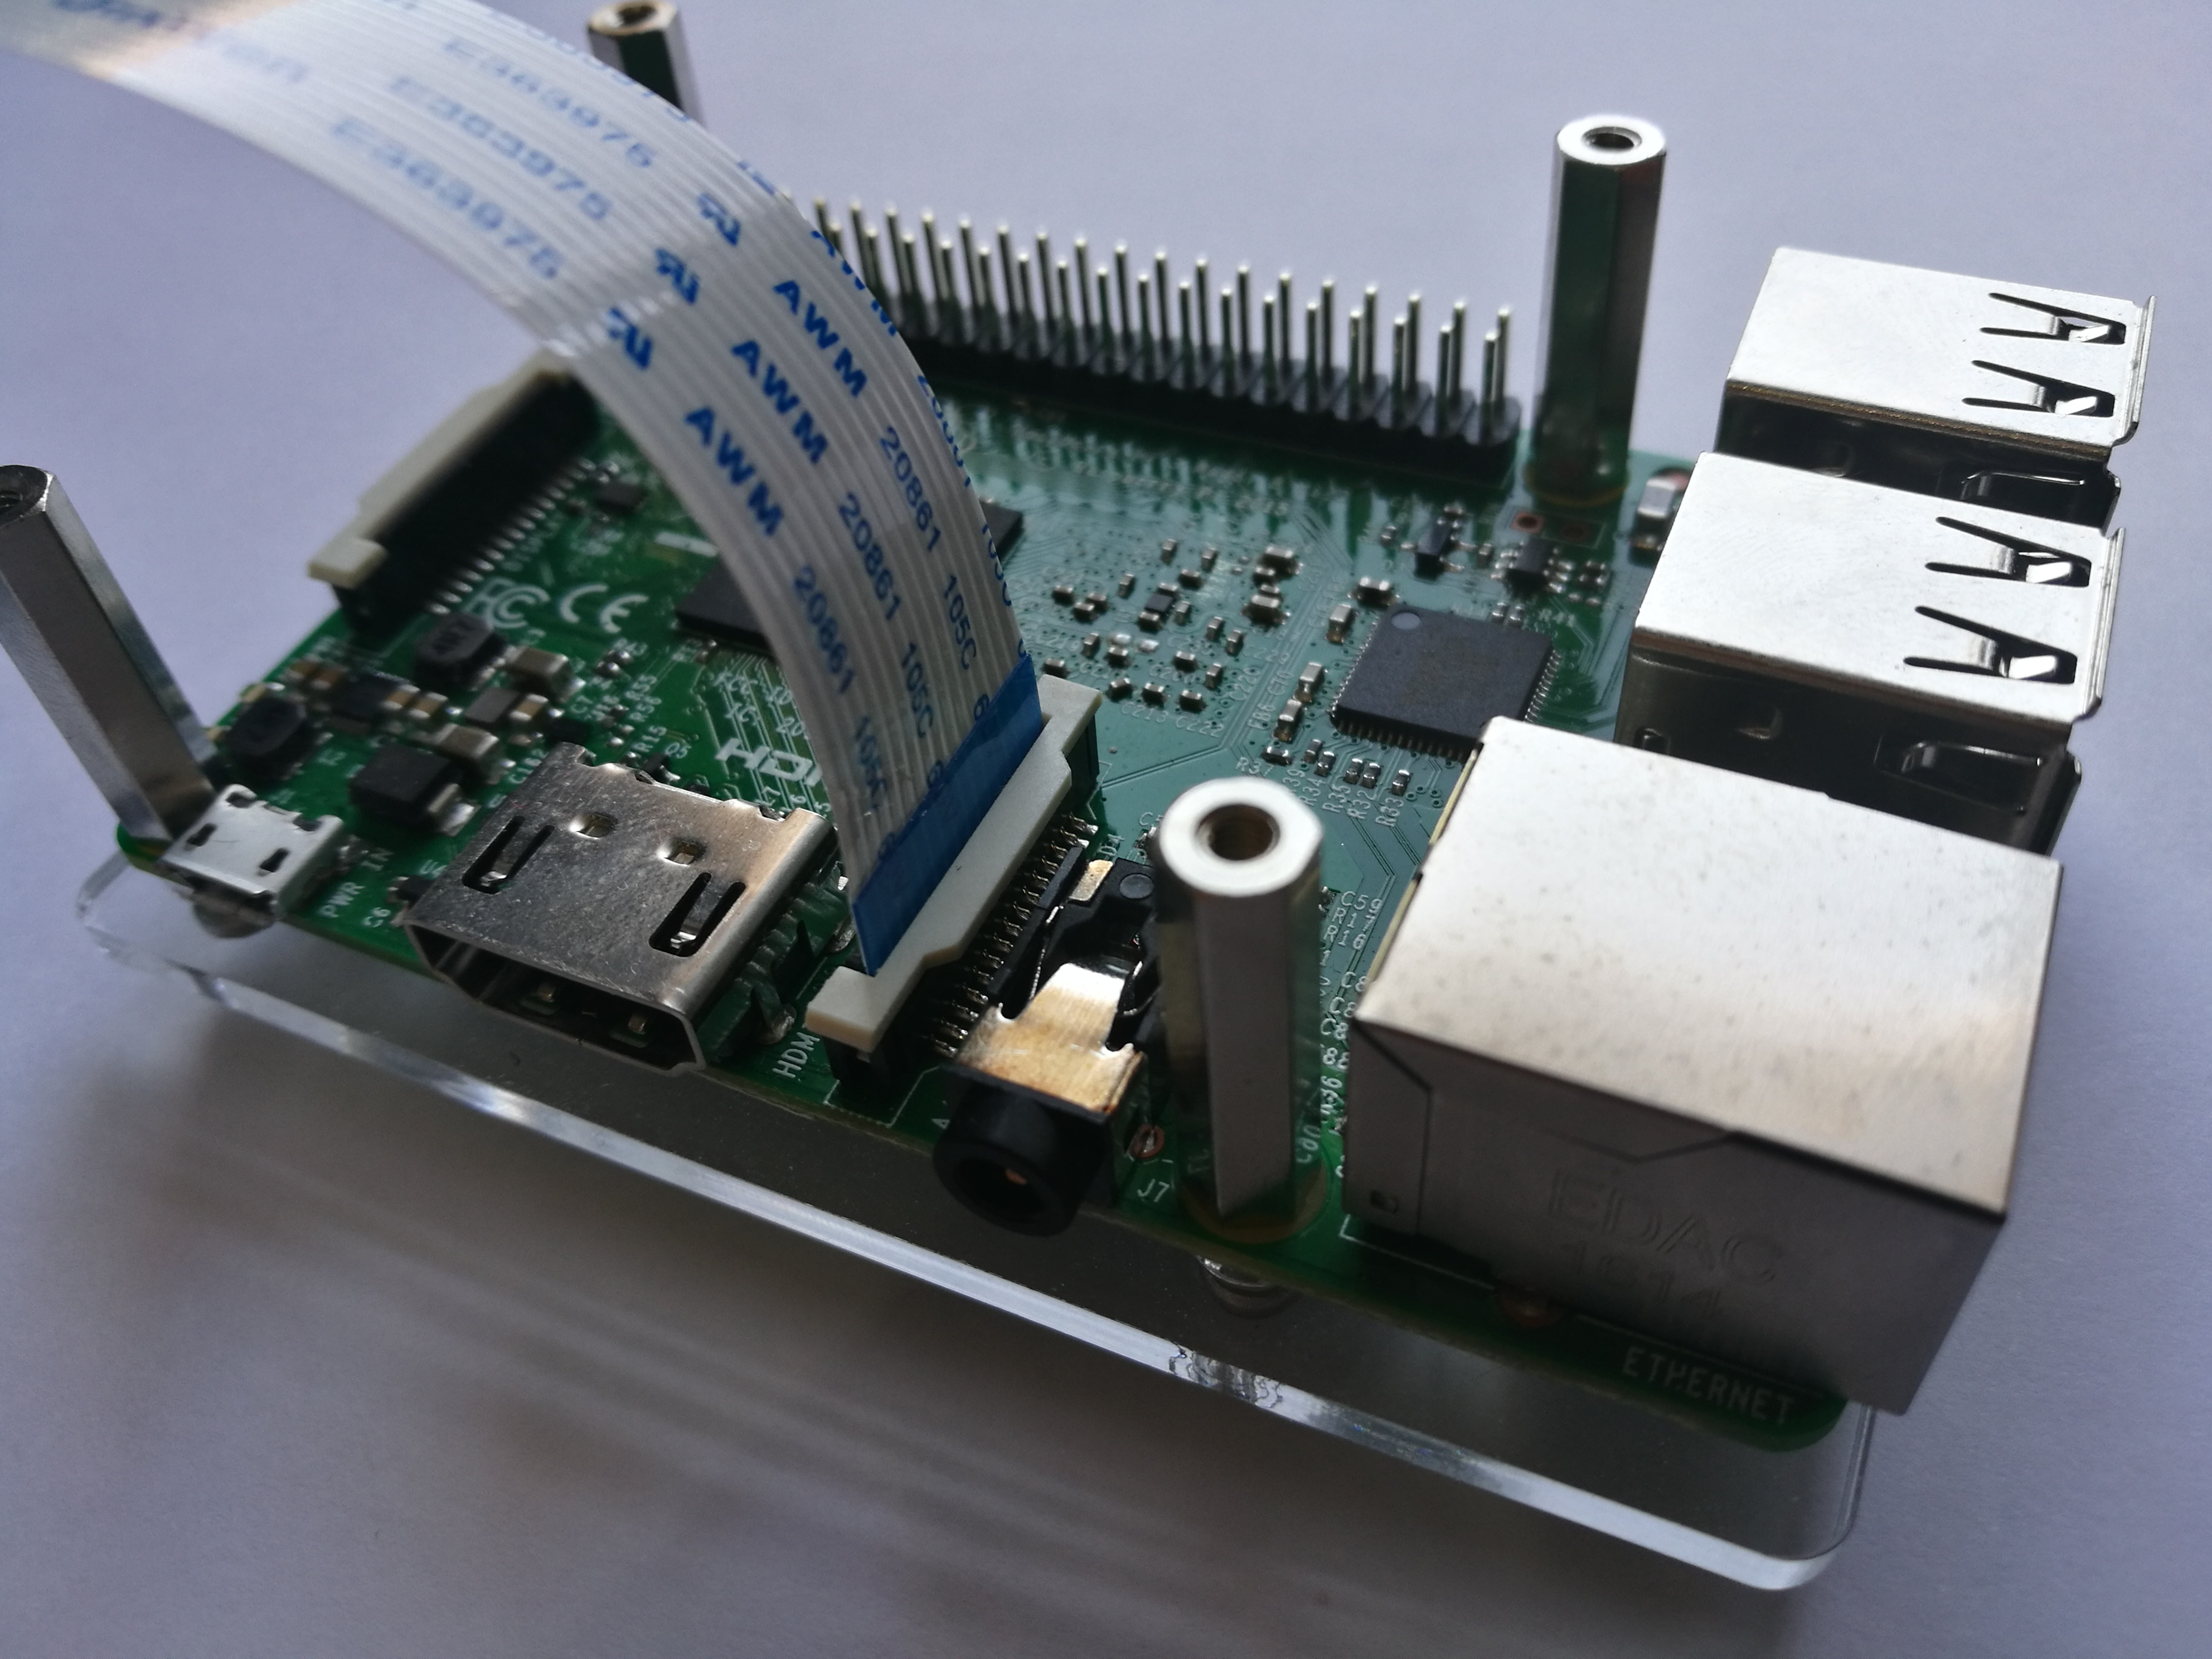
\includegraphics[width=0.75\textwidth]{Appendix_camera_conection.jpg}
		\caption{Connection of the camera module to the Raspberry Pi 3.}
		\label{fig:Appendix_camera_conection}
	\end{center}
\end{figure} %TODO: Cambiar imagen ?


\subsection{Installation of the sense hat}
The installation of the sense hat is explained on Task T2.4.1 of the Sprint 2 on the  \nameref{chap:results} chapter.

\subsection{Installation of the sensors}
The installation of the sense hat is explained on Tasks T2.4.2 and T2.5.1 of the Sprint 2 on the  \nameref{chap:results} chapter.


\subsection{Installation of the necessary libraries}
Some libraries are needed in order to execute the software developed in this \ac{BSc.} thesis:
\begin{enumerate}
	\item NumPy. Is the fundamental package for scientific computing with Python. NumPy can also be used as an efficient multi-dimensional container of generic data. To install it, the next command has to be executed:
\begin{console}
$ sudo apt-get install python-numpy python3-numpy
\end{console} %$

	\item Matplotlib. Is a library for the generation of graphic from data contained in list or arrays using Python programming language and the NymPy package. It provides a MATLAB-like interface. To install it, the next command has to be executed:
\begin{console}
$ sudo apt-get install python-matplotlib python3-matplotlib
\end{console} %$

	\item MP4Box. It can be used for performing many manipulations on multimedia files like AVI, MPG, TS, but mostly on ISO media files (e.g. MP4, 3GP). The justification for using it is that PiCamera generates the video recordings in \emph{h265} format. Therefore, this tool is used to convert videos from \emph{h265} to \emph{mp4}. The installation is done by executing the command:
\begin{console}
$ sudo apt-get install gpac
\end{console} %$
	Once installed, any video (named \texttt{video.h264}) can be converted from \emph{h265} to \emph{mp4} at 30 \ac{FPS} using:
\begin{console}
$ MP4Box -fps 30 -add video.h264 video.mp4
\end{console} %$

	\item Sense hat. To allow Raspberry Pi access the Sense Hat module, the corresponding library has to be installed:
\begin{console}
	$ sudo apt-get install sense-hat
\end{console} %$

	\item IBM Watson \ac{IoT} Platform. Some libraries are needed to allow Python to use the IBM Watson \ac{IoT} Platform services, which are used to send the sensor data to the Cloud. These libraries can be installed by executing the following commands:
\begin{console}
	$ sudo pip3 install ibmiotf
\end{console} %$

\end{enumerate}

When all these steps are completed, the Raspberry Pi is prepared for the correct execution of the software developed in this \ac{BSc.} thesis.

% TFG - José Ángel Martín Baos. Escuela Superior de Informática. 2018
%%%% CHAPTER: User Manual %%%
% !TeX spellcheck = en_GB
\chapter{Configuration file}
\label{chap:config_file}

\drop{I}{n} Appendix B the configuration file required by the program developed for the Raspberry Pi is explained. This configuration file is shown in Listing \ref{lst:B-config}, where lines from 1 to 18 define the Camera module configuration, lines from  21 to 70 define the Sensor module configuration, and lines from 73 to 75 define the communication module configuration.


\lstinputlisting[language=Python, texcl, firstline=11, texcl, caption = {Raspberry Pi program \texttt{config.py} file.}, label = lst:B-config]{code/B-config.py}


\backmatter
\bibliography{main}
\cleardoublepage

\end{document}
